% ==============================================================================
% TRABALHO DE CONCLUSÃO DE CURSO — evasão no 1º ano nos cursos de Ciências
% Exatas do CCE/UFES (campus Goiabeiras), coortes 2019--2024.
% Estrutura conforme o Art. 6º do regulamento de TCC.
% Formatação conforme o template do Departamento de Estatística
% (template_tex/main.tex).
% Compilar: latexmk main  (pdflatex, ver latexmkrc; figuras em EPS, convertidas
% na compilação; tabelas e figuras vêm de scripts/, ver run_all.sh)
% ==============================================================================

\documentclass[12pt,a4paper]{article}

\usepackage[utf8]{inputenc}
\usepackage[T1]{fontenc}
\usepackage{lmodern}
\usepackage[brazilian]{babel}
% Margens do template
\usepackage{fancyhdr, lastpage}
\setlength{\topmargin}{-0.5in}
\setlength{\headheight}{39pt}
\setlength{\oddsidemargin}{0.25in}
\setlength{\evensidemargin}{0.25in}
\setlength{\textwidth}{6.0in}
\setlength{\textheight}{8.5in}
\usepackage{titlesec}
\titleformat{\section}{\Large\bfseries}{\thesection.}{1em}{}
\titleformat*{\subsection}{\normalsize\bfseries}
\usepackage{tocloft}
\renewcommand{\cftdot}{}
\usepackage{pdfpages}
\usepackage{amsmath,amssymb}
\usepackage{booktabs}
\usepackage{array,tabularx}
\usepackage{makecell}
\usepackage{etoolbox}
\AtBeginEnvironment{table}{\small\setlength{\tabcolsep}{4pt}}
\setlength{\emergencystretch}{1.5em}
\usepackage{longtable}
\usepackage{graphicx}
\usepackage{caption}
\usepackage{float}
\usepackage{url}
\usepackage[authoryear,round]{natbib}
\usepackage{tikz}
\usetikzlibrary{positioning,arrows.meta}

\AtBeginEnvironment{tabular}{\small}
\setlength{\tabcolsep}{4pt}
\setlength{\parindent}{0pt}
\setlength{\parskip}{6pt minus 1pt}
\captionsetup{font=small,labelfont=bf,labelsep=period,justification=raggedright}

\graphicspath{{figuras/}{template_tex/}}
% As tabelas geradas foram dimensionadas para 16 cm; na mancha do template
% (6 in x 8,5 in), as que não cabem são reduzidas na proporção necessária.
\newsavebox\caixatabela
\newcommand{\tabela}[1]{\sbox\caixatabela{\input{tabelas/#1}}%
  \ifdim\wd\caixatabela>\linewidth \resizebox{\linewidth}{!}{\usebox\caixatabela}%
  \else\ifdim\dimexpr\ht\caixatabela+\dp\caixatabela\relax>0.80\textheight
    \resizebox*{!}{0.80\textheight}{\usebox\caixatabela}%
  \else\usebox\caixatabela\fi\fi}
% Título dos apêndices no sumário: "Apêndice A -- Título".
\newcommand\apendicetoc[1]{\appendixname~#1~--~}
\newcommand{\aredigir}[1]{\par\noindent\fbox{\parbox{0.95\linewidth}{\small\textit{#1}}}\par}

% Flutuantes perto da citação: mais flutuantes por página e menos texto exigido
\renewcommand{\topfraction}{0.85}
\renewcommand{\bottomfraction}{0.7}
\renewcommand{\textfraction}{0.1}
\renewcommand{\floatpagefraction}{0.75}
\setcounter{topnumber}{3}
\setcounter{bottomnumber}{2}
\setcounter{totalnumber}{5}

\begin{document}

% ==============================================================================
% I. CAPA
% ==============================================================================
\begin{titlepage}
\begin{flushright}
\LARGE{\textbf{Trabalho de Conclusão de Curso}}\\
\vfill
\LARGE{\textbf{Associação e capacidade de discriminação na evasão do curso no primeiro ano: características de ingresso pelo Sisu no~CCE/Ufes}}\\
\vfill

\large Aluna: Nathália Dantas Handam Nunes\\
\large Orientador: Fabio Alexander Fajardo Molinares\\
\vfill

\textbf{Departamento de Estatística}\\
Centro de Ciências Exatas\\
\today
\vfill

\includegraphics[width=0.25\linewidth]{LogoDeptEstatistica_final.png}\hspace{6,5cm}

\includegraphics[width=0.25\linewidth]{Logo_COLEST.png}\\
\end{flushright}
\end{titlepage}
\pagenumbering{roman}

% ==============================================================================
% II. RESUMO E ABSTRACT
% ==============================================================================
\section*{Resumo}
\addcontentsline{toc}{section}{Resumo}

Segundo os indicadores do Instituto Nacional de Estudos e Pesquisas Educacionais Anísio Teixeira (Inep), nos cursos de Ciências Exatas das universidades federais, a evasão no primeiro ano é maior do que nos demais cursos. Este estudo examina se as características registradas no ingresso pelo Sistema de Seleção Unificada (Sisu) e pelo Exame Nacional do Ensino Médio (Enem) (renda familiar; origem, que combina a escola e a modalidade de ingresso; nota de seleção; sexo; cor/raça) se associam à evasão no primeiro ano e quanto ajudam a distinguir quem sai de quem permanece. Evasão aqui é a saída formal do curso, o que inclui a troca de curso. Foram analisadas as 1.320 matrículas dos ingressantes de 2019 a 2024 nos sete cursos do Centro de Ciências Exatas da Universidade Federal do Espírito Santo (Estatística e os bacharelados e as licenciaturas em Física, Matemática e Química). Um quarto delas (25,2\%) terminou em evasão, a maioria no primeiro semestre. A associação foi medida pelo risco relativo, que diz quantas vezes o risco de evasão de um grupo é o de outro. Os riscos relativos vieram de uma regressão de Poisson modificada, que ajusta cada característica pelas demais. A capacidade de distinguir foi medida pela área sob a curva (AUC), a probabilidade de que, em um par formado por um estudante que saiu e outro que permaneceu, o modelo atribua maior risco ao primeiro. A AUC vale 0,5 quando o modelo não faz melhor que o acaso. A renda familiar teve indício fraco de associação, com risco maior nas rendas mais baixas. Esse indício deve ser tratado como hipótese, porque o modo de incluir a renda no modelo foi escolhido depois de explorados os dados. Trata-se também de um achado frágil, pois a evidência ficou ainda mais fraca sem a coorte de 2024 e com outros métodos de estimação. Para a nota de seleção, a origem, o sexo e a cor/raça, os dados não permitem afirmar nem descartar associação. Somadas, as características de ingresso quase não melhoraram essa distinção, pois a AUC, descontado o ganho artificial de avaliar o modelo nos dados em que foi ajustado, passou de 0,518, em um modelo só com curso e coorte, para 0,541. A evasão foi parecida nos sete cursos, de 21,1\% a 27,4\%. Em uma análise exploratória, a renda pareceu pesar mais nas três licenciaturas e no bacharelado em Estatística do que nos bacharelados em Física, Matemática e Química. No momento da matrícula, portanto, o perfil de ingresso pouco antecipa a evasão precoce nesses cursos.

\noindent\textbf{Palavras-chave:} evasão no ensino superior; Ciências Exatas;
Sisu/Enem; ações afirmativas; regressão de Poisson modificada.

\newpage
\section*{Abstract}
\addcontentsline{toc}{section}{Abstract}

According to the indicators of the National Institute for Educational Studies and Research Anísio Teixeira (Inep), first-year dropout in the Exact Sciences programs of Brazilian federal universities is higher than in other programs. This study examines whether the characteristics recorded at entry by the Unified Selection System (Sisu) and the National High School Exam (Enem) (family income; origin, which combines school and admission category; admission score; sex; race/color) are associated with first-year dropout and how much they help to tell apart students who leave from those who stay. Dropout here means formally leaving the program, which includes switching programs. The analysis covered the 1,320 enrollments of students admitted from 2019 to 2024 to the seven programs of the Center for Exact Sciences of the Federal University of Espírito Santo (Statistics and the bachelor's and teaching degrees in Physics, Mathematics and Chemistry). One in four (25.2\%) ended in dropout, most of them in the first semester. Association was measured by the relative risk, which states how many times the dropout risk of one group is that of another. Relative risks came from a modified Poisson regression, which adjusts each characteristic for the others. The ability to tell students apart was measured by the area under the curve (AUC), the probability that, in a pair formed by a student who left and one who stayed, the model assigns a higher risk to the former. The AUC equals 0.5 when the model does no better than chance. Family income showed a weak indication of association, with higher risk at lower incomes. This indication should be treated as a hypothesis, because the way income enters the model was chosen after the data had been explored. It is also a fragile finding, as the evidence became even weaker without the 2024 cohort and with other estimation methods. For admission score, origin, sex and race/color, the data neither establish nor rule out an association. Taken together, entry characteristics barely improved this ability, as the AUC, net of the artificial gain of evaluating the model on the data used to fit it, went from 0.518, in a model with program and cohort only, to 0.541. Dropout was similar across the seven programs, from 21.1\% to 27.4\%. In an exploratory analysis, income seemed to weigh more in the three teaching degrees and in the Statistics bachelor's degree than in the Physics, Mathematics and Chemistry bachelor's degrees. At enrollment, therefore, the entry profile barely anticipates early dropout from these programs.

\noindent\textbf{Keywords:} higher education dropout; Exact Sciences;
Sisu/Enem; affirmative action; modified Poisson regression.

% ==============================================================================
% III. DECLARAÇÃO DE USO DE INTELIGÊNCIA ARTIFICIAL
% ==============================================================================
% Formulário do colegiado (declaracao_de_uso_de_ai.pdf). O latexmkrc gera a
% cópia _flat, com os campos preenchidos e a assinatura fixados na página;
% para assinar, basta trocar o PDF original e compilar de novo.
\includepdf[pages=-,pagecommand={\thispagestyle{empty}\addcontentsline{toc}{section}{Declaração de uso de Inteligência Artificial}}]{declaracao_de_uso_de_ai_flat.pdf}

\newpage
\tableofcontents
\newpage
\listoffigures
\newpage
\listoftables
\newpage
% ==============================================================================
% IV. INTRODUÇÃO
% ==============================================================================
\clearpage
\pagenumbering{arabic}
\section{Introdução}
\label{sec:introducao}

A expansão do ensino superior público mudou o perfil de quem chega às universidades públicas brasileiras, federais e estaduais. Segundo \citet{costaTD2631Expansao2021}, entre 2005 e 2015 essas universidades receberam uma parcela crescente de estudantes de baixa renda, pretos e pardos. Nas federais, a Lei 12.711, de 2012, reservou metade das vagas a egressos de escola pública, com subcotas por renda e por cor/raça \citep{brasil2012lei12711}. Ampliar o ingresso, no entanto, não garante a permanência. A partir de 2007, o Programa de Apoio a Planos de Reestruturação e Expansão das Universidades Federais (Reuni) ampliou as vagas dessas instituições. Entre as suas diretrizes, incluiu a redução da evasão sem definir o termo, o que deixou a cada instituição federal a tarefa de defini-lo \citep[p.~6]{coimbraEvasaoNaEducacao2021}.

Na literatura, os critérios que definem a evasão também variam de um estudo para outro e quase nunca se diferenciam pela causa da perda do vínculo (\citealp[p.~3]{coimbraEvasaoNaEducacao2021}; \citealp[p.~11]{starkEvasaoNoEnsino2025}). A Comissão Especial de Estudos sobre a Evasão do Ministério da Educação (MEC) distingue três saídas: a do curso, a da instituição e a do sistema de ensino superior. Só nesta última o estudante deixa de estudar \citep{coimbraEvasaoNaEducacao2021}. Este estudo adota a evasão do curso de ingresso \citep{arantesEvasaoRetencaoNo2021}, isto é, a saída do curso em que o estudante foi admitido, permaneça ele ou não no ensino superior. É nesse nível que o curso perde o estudante. É também o único nível observável nos registros administrativos, que informam a forma da saída, mas não o destino de quem sai. Assim, quem muda de curso conta como evadido, mesmo quando a troca o leva a um curso mais adequado, como nos indicadores de trajetória do Instituto Nacional de Estudos e Pesquisas Educacionais Anísio Teixeira (Inep). Como neles, a matrícula trancada conta como permanência \citep{inep2017metodologia}.

Com os microdados do Censo da Educação Superior, \citet{gomesDeterminantesEvasaoNo2024} acompanharam a coorte nacional de ingressantes de 2010 até 2017. Ao fim do quarto ano, 42\% dos estudantes já haviam deixado o curso. Nas Ciências Exatas, o quadro é mais grave desde o início do curso. Em 2005, o curso de Matemática já tinha a maior taxa anual de evasão do país, 44\% \citep{silvafilhoEvasaoNoEnsino2007}. Pelos indicadores de trajetória do Inep, entre os ingressantes de 2019 nos cursos presenciais de Matemática, Física, Química e Estatística das universidades federais, 12,5\% deixaram o curso ainda no ano de ingresso, contra 7,2\% nos demais cursos. Até o fim do segundo ano, a proporção chegou a 25,5\%, contra 15,5\%. Até o quinto, chegou a 55\% \citep{inep2025trajetoria}. O primeiro ano responde por menos de um quarto dessa perda. Mesmo assim, é nele que algumas características de ingresso mais se associaram à saída em dois estudos que estimaram essa associação ano a ano. Em uma universidade pública de quatro anos do Meio-Oeste dos Estados Unidos, que o autor não identifica, a renda familiar baixa e as notas do ensino médio perderam associação com a saída da instituição depois do primeiro ano \citep{ishitani2003longitudinal}. Na Universidade Federal do Rio de Janeiro (UFRJ), não ter ingressado na primeira opção de curso, ou ter a escolha afetada pela nota de corte, associou-se à evasão sobretudo nesse ano \citep{klitzkeFATORESASSOCIADOSEVASAO2023}. Quanto mais longo o horizonte, mais a trajetória no curso se interpõe entre o registro de ingresso e a saída. Por isso, o desfecho é a evasão até o fim do primeiro ano acadêmico, horizonte idêntico para todas as coortes analisadas.

O modelo de integração do pesquisador estadunidense Vincent \citet{tintoDropoutHigherEducation1975}, que organiza a trajetória do estudante em estágios, é o referencial mais citado nos estudos brasileiros sobre o tema \citep{starkEvasaoNoEnsino2025}. No primeiro estágio, a origem familiar, a escolarização prévia e as características individuais definem o compromisso inicial do estudante. Segundo o autor, a decisão de permanecer ou sair se constrói depois, na integração acadêmica e social dos primeiros meses (\citealp[p.~8]{tinto1982defining}; \citealp{pinheiroModelosTeoricosEvasao2023,pradoPermanenciaNaEducacao2022}). Em 1988, o autor deu ao modelo uma dimensão temporal. Antes de se tornar membro da comunidade universitária, o ingressante passa pelas fases de separação e de transição, que se concentram no primeiro ano \citep[pp.~445, 451]{tinto1988stages}. Muitos estudantes saem na transição, mais pelo peso da passagem do que por falta de integração \citep[p.~444]{tinto1988stages}. Alain \citet[p.~1243]{coulon2017oficio}, que acompanhou estudantes de primeiro ano em universidades francesas, chama esse ano de ``tempo de todos os perigos''. Nele o estudante precisa se afiliar à universidade, isto é, adquirir o estatuto de estudante e decifrar as regras do novo meio \citep[p.~1247]{coulon2017oficio}. Para os dois autores, portanto, o primeiro ano, o mesmo coberto pelo desfecho, é o da passagem à vida universitária. Modelos posteriores ampliaram o papel dos fatores externos à instituição, que Tinto limitava à formação dos compromissos. No de \citet[pp.~132--135]{cabrera1993college}, o incentivo da família e dos amigos e a satisfação com o apoio financeiro agem também sobre a integração. Em um estudo anterior, \citet{cabrera1992role} associaram ter recebido ajuda financeira a maior integração social e a notas mais altas no primeiro ano.

A literatura nacional ressalta a necessidade de adaptar o modelo a um país de desigualdades socioeconômicas profundas, nas quais as condições de origem seguem atuando sobre a permanência \citep{pinheiroModelosTeoricosEvasao2023}. O modelo de Tinto serve aqui para delimitar o que os dados permitem ver. O cadastro do Sistema de Seleção Unificada (Sisu) e o questionário do Exame Nacional do Ensino Médio (Enem) registram o primeiro estágio, as características de ingresso. A integração posterior fica fora dos dados por dois motivos. O primeiro é que o histórico acadêmico registra reprovações e trancamentos, não a participação do estudante na vida acadêmica e social. Mesmo a reprovação só é lançada ao fim do semestre, ao mesmo tempo que a saída de quem deixou o curso. O segundo é que o apoio financeiro recebido depois da matrícula, que o modelo de Cabrera inclui, também não consta dos registros. Por isso, os dados permitem saber quanto da evasão já se distingue no momento da matrícula, mas não testar o modelo de Tinto.

Os estudos com dados institucionais oferecem evidência indireta sobre quanto as características de ingresso distinguem quem sai. Em modelos preditivos desenvolvidos na Universidade Federal de São João del-Rei (UFSJ) e em uma universidade pública do interior do Rio Grande do Sul, que os autores não identificam, as variáveis da trajetória acadêmica, como disciplinas cursadas e reprovadas, pesaram mais do que as notas do Enem e os dados de ingresso \citep{felizardoAnaliseDiscriminanteProbabilidade2023,salaberriMineracaoDadosEducacionais2024}. Esses trabalhos diferem em população, desfecho e método. Associações ajustadas do perfil de ingresso com a evasão também foram estimadas em universidades federais, com outros recortes. Na Universidade Federal do Recôncavo da Bahia (UFRB), com a evasão no primeiro semestre como desfecho e sem a renda nem a escola de origem entre as variáveis, ser cotista associou-se a mais evasão no Centro de Ciências Exatas e Tecnológicas, que inclui as Engenharias, mas não no conjunto da universidade \citep{lopes2023calouros}. Na Universidade Federal de Minas Gerais (UFMG), entre ingressantes de 2012 seguidos por sete anos, admitidos antes da adesão ao Sisu e da Lei 12.711, os egressos de escola pública federal evadiram do curso em proporção parecida com a dos de escola privada, também no modelo ajustado \citep{paula2025evasao}.

Entre os estudos lidos\footnote{Boa parte dos estudos empíricos citados foi localizada nas revisões sistemáticas de \citet{starkEvasaoNoEnsino2025}, com busca no SciELO, na Scopus, na Web of Science e na EBSCO por artigos de 2020 a 2024 e de \citet{mancano2026revisao}, com busca no Portal de Busca Integrada da USP pelos termos ``evasão'' e ``superior'' em artigos de 2010 a 2024. Os demais vêm das referências desses estudos e de publicações posteriores. Da segunda revisão, que reuniu 16 estudos com acompanhamento longitudinal e modelo multivariado, foram lidos todos os que estimam associações ajustadas com a evasão em cursos presenciais de universidades federais \citep{costa2020alem,rosa2021acesso,rosa2022prestigio,nierotkaAcessoEvasaoConclusao2023,nierotkaFatoresAssociadosEvasao2023,lopes2023calouros,klitzkeFATORESASSOCIADOSEVASAO2023,pereira2024evasao}.}, nenhum mediu quanto as características de ingresso acrescentam à discriminação sobre o que o curso e a coorte já informam. Em vez de prever a evasão com todas as informações disponíveis, inclusive as da trajetória no curso, como fazem os estudos preditivos, este estudo mede quanto as características de ingresso, somadas, melhoram a discriminação de um modelo que já contém o curso e a coorte. Medir a discriminação não é o mesmo que medir a associação, porque uma característica pode se associar à evasão e, ainda assim, pouco ajudar a distinguir quem sai, quando o risco maior se restringe a um grupo pequeno ou quando, mesmo nesse grupo, a maioria permanece.

Depois que a Lei 12.711 estendeu a reserva de vagas a todas as federais, por escola de origem, renda e cor/raça, os estudos passaram a comparar cotistas e não cotistas. Os resultados divergem. Em artigo na revista \textit{Avaliação}, \citet{andriolaImpactosLeiCotas2023} compararam a evasão na Universidade Federal do Ceará (UFC) antes e depois da adoção das cotas. Depois da adoção, de 2013 a 2017, a taxa média de evasão foi maior entre os cotistas do que entre os não cotistas, em uma comparação sem ajuste por outras características; no conjunto da Universidade Estadual Paulista (Unesp), a evasão não se distinguiu entre as formas de ingresso \citep{massini-cagliariImpactoPoliticaReserva2021}. Em escala nacional, a renda e o apoio financeiro se associaram à permanência. \citet{paulaDESIGUALDADESAPOSACESSO2024} ligaram os microdados do Enem de 2013 aos do Censo da Educação Superior de 2014 a 2019. Nesse estudo, os estudantes com renda familiar de até um salário mínimo tiveram razão de chances de abandono do ensino superior de 1,63 em relação aos de renda acima de cinco salários mínimos. Quem recebeu apoio financeiro permaneceu mais \citep{saccaroFatoresAssociadosEvasao2019,gomesDeterminantesEvasaoNo2024}. Na escola de origem, a chance de evasão não diminuiu de modo uniforme da escola privada para a pública. Os egressos de escola pública federal tiveram chance de evasão 59\% menor do que os de escola privada. Os de escola estadual ou municipal tiveram chance só 3\% menor \citep{paulaDESIGUALDADESAPOSACESSO2024}. A modalidade de ingresso reúne estudantes de rendas diferentes, de modo que a comparação entre cotistas e não cotistas pode diluir uma associação com a renda. A comparação por renda talvez reflita a escola de origem. Essa possibilidade justifica examinar as duas características juntas, embora não baste para explicar a divergência entre os estudos.

Para associações fracas com a origem social entre universitários, três estudos brasileiros propõem a leitura da seleção na entrada, a partir de um argumento de \citet{mare1980social}. A cada etapa da escolarização, os estudantes de origem baixa que seguem adiante são mais selecionados em características não medidas, como habilidades e aspirações, do que os de origem alta. Por isso, a associação com a etapa seguinte se atenua em toda a escala, desde que o efeito daquelas características não mude de uma etapa para outra \citep[pp.~298--299]{mare1980social}. Assim \citet{nierotkaFatoresAssociadosEvasao2023} explicam a ausência de associação do nível socioeconômico com a evasão na Universidade Federal da Fronteira Sul (UFFS). \citet{klitzkeFATORESASSOCIADOSEVASAO2023} leem do mesmo modo a ausência de associação da origem sociodemográfica na UFRJ, depois de considerados os fatores educacionais e de escolha do curso. \citet[p.~14]{paulaDESIGUALDADESAPOSACESSO2024} usam o argumento para comparar instituições, pois a seleção por exames concorridos tornaria as desigualdades na evasão menores nas universidades federais e estaduais.

Outra chave para a relação entre origem social e trajetória escolar é o capital cultural, que, na sociologia de Pierre Bourdieu, inclui a informação sobre o funcionamento do sistema de ensino, decisiva para continuar os estudos, mudar de estabelecimento ou escolher o curso superior \citep{bourdieuPasseronReproducao,nogueira2002sociologia}. A escolaridade dos pais, seu indicador usual, mede só a forma institucionalizada desse capital, os títulos escolares \citep{nogueira2002sociologia}.

Este estudo responde a duas perguntas. A primeira é se as características registradas no ingresso pelo Sisu e pelo Enem (renda familiar; origem, que combina a modalidade de ingresso e o tipo de escola; nota de seleção; sexo; cor/raça) se associam à evasão do curso no primeiro ano. Essa primeira pergunta inclui saber qual, entre a renda e a origem, permanece associada quando a outra é levada em conta. A segunda é quanto essas características, somadas, acrescentam à discriminação entre quem evade e quem permanece, além do que o curso e a coorte já informam. O objetivo principal é estimar a associação ajustada dessas características com a evasão em riscos relativos, com renda e origem ajustadas uma pela outra. O objetivo secundário é medir o ganho de discriminação de um modelo com todas as características de ingresso sobre um modelo de referência com curso e coorte. A medida é a área sob a curva ROC (AUC, do inglês \textit{area under the curve}; ROC, de \textit{receiver operating characteristic}). A AUC estima a probabilidade de o modelo atribuir maior risco a quem evadiu do que a quem permaneceu.

As duas perguntas são examinadas nos cursos de graduação do Centro de Ciências Exatas (CCE) da Universidade Federal do Espírito Santo (Ufes), no campus de Goiabeiras. O CCE foi escolhido porque seus sete cursos de bacharelado e licenciatura cobrem Estatística, Física, Matemática e Química, as áreas cuja evasão no primeiro ano supera a dos demais cursos das universidades federais. Nos estudos nacionais e na UFFS, a licenciatura teve mais evasão do que o bacharelado \citep{gomesDeterminantesEvasaoNo2024,paulaDESIGUALDADESAPOSACESSO2024,nierotkaAcessoEvasaoConclusao2023}. Por isso, o curso entra no modelo. A população é composta pelos ingressantes por meio do Sisu no primeiro semestre das coortes de 2019 a 2024, que têm o mesmo registro de entrada, as notas e o questionário socioeconômico do Enem. O período começa em 2019, primeira coorte cujas saídas foram registradas pela mesma regra das coortes seguintes. Termina na última cujo Enem, edição de 2023, permite a ligação individual entre notas e questionário, porque a partir da edição de 2024 o Inep passou a publicar os dois em arquivos sem chave comum \citep{inep2025leiame}. Esse intervalo inclui o ensino remoto emergencial de 2020 e a greve de 2024. A estabilidade das associações é verificada sem essas coortes.

O texto está organizado em três partes. A Metodologia (Seção~\ref{sec:fundamentacao}) apresenta os fundamentos estatísticos da análise; as Aplicações (Seção~\ref{sec:aplicacoes}) descrevem os dados, os procedimentos de análise, os resultados e a discussão; e a Conclusão (Seção~\ref{sec:conclusao}) retoma a contribuição do estudo e seus limites.

% ==============================================================================
% V. METODOLOGIA
% ==============================================================================
\section{Metodologia}
\label{sec:fundamentacao}
\label{sec:fund-estatistica}

\subsection{Risco relativo e regressão de Poisson modificada}
\label{sec:fund-poisson}

Para cada matrícula $i = 1, \dots, n$, seja $Y_i$ a variável aleatória que vale 1 se a matrícula terminou em evasão no primeiro ano e 0 caso contrário. Seja $\mathbf{x}_i$ o vetor das suas covariáveis. Dado $\mathbf{x}_i$, $Y_i$ tem distribuição de Bernoulli com parâmetro $\pi_i = P(Y_i = 1 \mid \mathbf{x}_i)$, o risco de evasão da matrícula. As matrículas são tratadas como independentes, o que exige verificar a dependência entre as matrículas de uma mesma pessoa.

A chance de evasão é a razão $\pi_i/(1-\pi_i)$ entre a probabilidade de evadir e a de permanecer. A regressão logística modela o seu logaritmo, $\operatorname{logit}(\pi_i) = \log\{\pi_i/(1-\pi_i)\} = \mathbf{x}_i^\top\boldsymbol{\beta}$. Nela, $e^{\beta_j}$ é a razão de chances (OR, do inglês \textit{odds ratio}) associada a um acréscimo de uma unidade em $x_{ij}$, mantidas as demais covariáveis. Sendo $\pi_0$ e $\pi_1$ os riscos de dois grupos, o risco relativo é $\text{RR} = \pi_1/\pi_0$. As duas medidas se relacionam por

\begin{equation}
  \text{OR} = \text{RR} \times \frac{1 - \pi_0}{1 - \pi_1}.
\end{equation}
Quando o desfecho é raro, os dois termos $1 - \pi$ ficam perto de 1. A OR se aproxima do RR. Quando é frequente, as duas medidas se afastam. Com riscos de 0,30 e 0,20, por exemplo, o RR é 1,50 e a OR, 1,71. Quando o desfecho é frequente, a OR exageraria as associações se fosse lida como RR \citep{zou2004modified}.

Para estimar o RR diretamente, troca-se a ligação logit pela logarítmica, $\log \pi_i = \mathbf{x}_i^\top\boldsymbol{\beta}$, em que $e^{\beta_j}$ é o RR associado a um acréscimo de uma unidade em $x_{ij}$, mantidas as demais covariáveis. Na regressão de Poisson modificada, esse modelo é ajustado ao desfecho binário como se ele tivesse distribuição de Poisson, isto é, os parâmetros $\boldsymbol{\beta}$ são estimados resolvendo as equações de estimação do modelo de Poisson,

\begin{equation}
  \sum_{i=1}^{n} \mathbf{x}_i \left(y_i - e^{\mathbf{x}_i^\top\boldsymbol{\beta}}\right) = \mathbf{0}. \label{eq:score}
\end{equation}
Embora $Y_i$ não tenha distribuição de Poisson, o estimador $\hat{\boldsymbol{\beta}}$ é consistente desde que a forma suposta para a média, $\log \pi_i = \mathbf{x}_i^\top\boldsymbol{\beta}$, seja a verdadeira \citep{zou2004modified,spiegelman2005easy}, ainda que a variância suposta esteja errada \citep[pp.~128, 279]{agresti2015foundations}.

O que a distribuição suposta afeta é a variância. A de Poisson, $\pi_i$, difere da de Bernoulli, $\pi_i(1-\pi_i)$. Por isso, a fórmula usual da covariância de $\hat{\boldsymbol{\beta}}$ deixa de valer e é substituída pelo estimador sanduíche \citep[p.~280]{agresti2015foundations},

\begin{equation}
  \widehat{\operatorname{Var}}(\hat{\boldsymbol{\beta}}) = \mathbf{A}^{-1}\mathbf{M}\mathbf{A}^{-1}, \quad \mathbf{A} = \sum_{i} \hat{\pi}_i \mathbf{x}_i\mathbf{x}_i^\top, \quad \mathbf{M} = \sum_{i} \frac{(y_i - \hat{\pi}_i)^2}{(1 - h_{ii})^2}\, \mathbf{x}_i\mathbf{x}_i^\top,
\end{equation}
com $\hat{\pi}_i = e^{\mathbf{x}_i^\top\hat{\boldsymbol{\beta}}}$ o risco predito da matrícula $i$. Na expressão de $\mathbf{M}$, $h_{ii}$ é a alavancagem da matrícula $i$, o elemento diagonal da matriz de projeção do ajuste, $\mathbf{H} = \boldsymbol{\Omega}^{1/2}\mathbf{X}(\mathbf{X}^\top\boldsymbol{\Omega}\mathbf{X})^{-1}\mathbf{X}^\top\boldsymbol{\Omega}^{1/2}$, em que $\mathbf{X}$ é a matriz cujas linhas são os $\mathbf{x}_i^\top$ e $\boldsymbol{\Omega}$ é a matriz diagonal dos pesos do ajuste, que no modelo de Poisson com ligação logarítmica são os $\hat{\pi}_i$. As alavancagens ficam entre 0 e 1 e somam o número de parâmetros \citep[pp.~127, 136--138]{agresti2015foundations}. O denominador $(1-h_{ii})^2$ é a correção para amostra finita da forma HC3 do estimador consistente sob heteroscedasticidade (HC, do inglês \textit{heteroskedasticity-consistent}) \citep{zeileis2004econometric,zeileis2006object}, que infla a contribuição das observações de alta alavancagem. Nas simulações de \citet[pp.~217, 222--223]{long2000using}, feitas com regressão linear para comparar as formas HC0 a HC3, que diferem na correção dos resíduos pela alavancagem, essa forma foi a recomendada para amostras de até 250 observações. A partir de 500 as formas quase não diferiram. Como infla mais os resíduos das observações de alta alavancagem, a HC3 dá os maiores erros-padrão entre as formas e, nas mesmas simulações, foi a de menor poder \citep[pp.~221--222]{long2000using}. Em amostras maiores, ela é, portanto, a escolha conservadora.

O RR estimado é $e^{\hat\beta_j}$ e o intervalo de confiança de 95\%, $\exp(\hat\beta_j \pm 1{,}96\,\widehat{\text{ep}}_j)$, em que $1{,}96 = \Phi^{-1}(0{,}975)$ e o erro-padrão $\widehat{\text{ep}}_j$ é a raiz do $j$-ésimo elemento da diagonal de $\widehat{\operatorname{Var}}(\hat{\boldsymbol{\beta}})$. Como a ligação logarítmica não restringe $\hat{\pi}_i$ ao intervalo $[0, 1]$, essa condição precisa ser verificada nos dados.

\subsection{Testes e leitura dos valores p}
\label{sec:fund-testes}

Para uma variável com $k$ categorias, representada por $k-1$ coeficientes $\boldsymbol{\beta}_{(k-1)}$, a hipótese de que nenhuma categoria difere da referência, $H_0: \boldsymbol{\beta}_{(k-1)} = \mathbf{0}$, é testada pela estatística de Wald

\begin{equation}
  W = \hat{\boldsymbol{\beta}}_{(k-1)}^\top \widehat{\mathbf{V}}^{-1} \hat{\boldsymbol{\beta}}_{(k-1)},
\end{equation}
em que $\widehat{\mathbf{V}}$ é o bloco da matriz sanduíche correspondente a esses coeficientes. Sob $H_0$, $W$ segue assintoticamente uma distribuição qui-quadrado com $k-1$ graus de liberdade, isto é, a distribuição de $W$ se aproxima dela à medida que $n$ cresce. O valor p calculado por ela é, por isso, aproximado \citep[pp.~129--131, 280]{agresti2015foundations}. Por testar de uma vez todas as categorias de uma variável, esse teste é chamado aqui de teste global. A mesma estatística testa juntos os coeficientes de um \textit{spline} ou de um conjunto de termos de interação.

O valor p de cada teste indica quão incompatíveis os dados são com a hipótese nula, dado o modelo, mas não mede o tamanho da associação, pois estimativas iguais dão valores p diferentes quando a precisão difere. Um valor p alto não é evidência de que a associação seja nula \citep[p.~341]{wasserstein2016asa,greenland2016statistical}. Por isso, a conclusão não deveria depender de um limiar rígido, como se uma associação passasse a existir de um lado de 0,05 e deixasse de existir do outro. Como alternativa, \citet{muff2022rewriting} propõem uma linguagem gradual de evidência, em faixas aproximadas do valor p (pouca ou nenhuma evidência acima de 0,10, evidência fraca de 0,10 a 0,05, moderada de 0,05 a 0,01, forte de 0,01 a 0,001 e muito forte abaixo disso), cujas fronteiras não devem ser tomadas como limiares.

Pela mesma razão, a comparação entre resultados não se faz pelos valores p. Dois valores p próximos, vindos de testes com graus de liberdade e precisões diferentes, não ordenam as associações que testam. Também a passagem de um valor p de um lado a outro de 0,05, de uma análise para outra, pode corresponder a uma mudança pequena e não significante na associação estimada. Comparar as duas análises exige estimar e testar a diferença entre elas \citep{gelman2006difference}. Comparar duas categorias de uma variável pelos seus contrastes com a referência tampouco testa a diferença entre elas. Esses contrastes são correlacionados, porque todos dependem da precisão da categoria de referência. A diferença se estima e se testa pelo contraste direto entre as duas (\citealp[p.~1025]{easton1991floating}; \citealp[pp.~329--330]{gelman2006difference}).

O poder de um teste, a probabilidade de rejeitar a hipótese nula quando ela é falsa, serve ao planejamento, porque descreve o que um desenho permite distinguir. Para uma covariável binária presente em $n_1$ de $n$ matrículas, com risco $\pi_0$ nas $n_0 = n - n_1$ demais e $\pi_1 = \text{RR}\,\pi_0$ nas $n_1$, a variância do logaritmo do RR estimado é aproximadamente

\begin{equation}
  \operatorname{Var}(\log \widehat{\text{RR}}) \approx \frac{1-\pi_1}{n_1\pi_1} + \frac{1-\pi_0}{n_0\pi_0}. \label{eq:poder}
\end{equation}
O teste bilateral de nível $\alpha$ tem poder $1-\gamma$ para o RR em que $|\log \text{RR}| = \{\Phi^{-1}(1-\alpha/2) + \Phi^{-1}(1-\gamma)\}\{\operatorname{Var}(\log \widehat{\text{RR}})\}^{1/2}$, em que $\Phi^{-1}$ é a inversa da função de distribuição da normal padrão, desprezada a rejeição na direção oposta. Depois da análise, o poder não acrescenta ao valor p, pois, avaliado no efeito estimado, é função do próprio valor p. O efeito detectável calculado com a variabilidade observada leva a conclusões que contradizem os valores p \citep{hoenig2001abuse}. Os valores da associação compatíveis com os dados são os do intervalo de confiança, cuja largura mede a precisão.

Quando se fazem vários testes, cada um ao nível $\alpha$, controla-se a taxa de erro de cada comparação, a probabilidade de rejeitar naquele teste uma hipótese nula verdadeira. A taxa de erro do conjunto, a probabilidade de ao menos uma rejeição falsa entre todos os testes, cresce com o número deles. Com $J$ testes independentes e todas as hipóteses nulas verdadeiras, ela vale $1-(1-\alpha)^J$ e, com testes correlacionados, depende da correlação entre eles. Controlá-la exige ajustar os níveis, como fazem os métodos de Bonferroni e de Holm. Qual das duas taxas controlar depende da pergunta. Em um estudo confirmatório em que uma conclusão única se apoia em vários testes, o ajuste é indispensável. Quando as análises são guiadas pelos dados, os resultados são exploratórios e servem para gerar hipóteses, com ou sem ajuste. Em qualquer caso, declaram-se a taxa controlada e o motivo da escolha \citep{bender2001adjusting}.

\subsection{Verificação do estimador e colinearidade}
\label{sec:fund-verificacao}

O modelo log-binomial usa a mesma ligação, $\log \pi_i = \mathbf{x}_i^\top\boldsymbol{\beta}$, mas supõe para $Y_i$ a distribuição de Bernoulli e estima $\boldsymbol{\beta}$ por máxima verossimilhança. Quando o ajuste chega ao máximo, esse é o estimador mais eficiente. O de Poisson modificado, embora válido, não é plenamente eficiente em relação a ele \citep{spiegelman2005easy}. O máximo é procurado por um algoritmo iterativo, que parte de valores iniciais e os corrige a cada passo até que as estimativas deixem de mudar. É isso que se chama convergir. A dificuldade está no espaço dos parâmetros. Como os riscos são probabilidades, a verossimilhança só existe se $e^{\mathbf{x}_i^\top\boldsymbol{\beta}} < 1$ para toda matrícula e, quando o máximo fica perto dessa fronteira, o algoritmo falha ou só converge a partir de valores iniciais escolhidos com cuidado \citep{zou2004modified}. Os dois modelos têm a mesma forma para a média e diferem só na estimação e na variância. Por isso, ajustá-los aos mesmos dados e comparar estimativas, resíduos e calibração mostra se a escolha entre eles muda a leitura.

Quando duas covariáveis do modelo se associam entre si, o ajuste de uma pela outra aumenta a variância das estimativas de ambas. Para um coeficiente isolado, esse aumento é medido pelo fator de inflação da variância, $\text{VIF}_j = 1/(1 - R_j^2)$, em que $R_j$ é a correlação múltipla da regressão da covariável $j$ nas demais \citep[p.~432]{fox2019companion}. O intervalo de confiança se alarga na proporção da sua raiz quadrada. Quando um termo ocupa vários coeficientes, como um \textit{spline} ou uma covariável categórica, o VIF de cada coeficiente depende da base escolhida para representá-lo. O fator generalizado (GVIF) de \citet{fox1992generalized} compara o volume da região de confiança conjunta dos coeficientes de um termo com o que ela teria se o termo fosse não correlacionado com as demais covariáveis,

\begin{equation}
  \text{GVIF} = \frac{\det \mathbf{R}_{11}\, \det \mathbf{R}_{22}}{\det \mathbf{R}},
\end{equation}
em que $\mathbf{R}$ é a matriz de correlação sem o intercepto, $\mathbf{R}_{11}$ o seu bloco do termo e $\mathbf{R}_{22}$ o das demais covariáveis. O GVIF vale 1 sem correlação e não depende da base. Para comparar termos com números diferentes de coeficientes, os autores propõem $\text{GVIF}^{1/(2p)}$, com $p$ o número de coeficientes do termo, que se lê como o aumento médio do erro-padrão e, com $p = 1$, é a raiz do VIF usual. A definição é do modelo linear, em que $\mathbf{R}$ é a correlação entre as covariáveis. Essa definição se aplica também aos modelos lineares generalizados, como o de Poisson \citep[pp.~432--434]{fox2019companion}. Na implementação do pacote car \citep{fox2026car}, seguida aqui, $\mathbf{R}$ é a correlação entre as estimativas dos coeficientes, que no modelo linear dá o mesmo valor; no modelo de Poisson, ela incorpora os pesos do ajuste.

\subsection{Diagnóstico e ajuste do modelo}
\label{sec:fund-diagnostico}

A influência de uma observação mede quanto as estimativas mudariam sem ela. A distância de Cook resume essa mudança para todos os coeficientes juntos, na métrica da região de confiança deles \citep[p.~16]{cook1977detection}. Ela foi definida para a regressão linear. Nos modelos lineares generalizados, a sua versão combina o resíduo padronizado $r_i$ e a alavancagem, $r_i^2\,h_{ii}/\{p(1-h_{ii})\}$, com $p$ o número de coeficientes \citep[p.~138]{agresti2015foundations}. O DFBETA olha um coeficiente de cada vez. É a diferença entre o coeficiente estimado com todas as observações e o estimado sem a observação $i$, que, dividida pelo erro-padrão do coeficiente, se lê em erros-padrão \citep[pp.~402--403]{fox2019companion}.

Três diagnósticos examinam se a forma suposta para a média, $\log \pi_i = \mathbf{x}_i^\top\boldsymbol{\beta}$, é adequada. O teste da ligação acrescenta ao modelo o quadrado do preditor linear estimado, $(\mathbf{x}_i^\top\hat{\boldsymbol{\beta}})^2$, cujo coeficiente é então testado. Esse termo, proposto por Tukey (1949 \textit{apud} \citealp[p.~23]{pregibon1980goodness}), costuma ser o mais sensível a desvios do modelo, sem indicar qual correção fazer. A soma de quadrados não ponderada dos resíduos, $\sum_i (y_i - \hat\pi_i)^2$, proposta por Copas (1989 \textit{apud} \citealp{hosmer1997comparison}), compara o ajuste ao que se espera sob o modelo. Os resíduos parciais de uma covariável somam ao resíduo de trabalho, $(y_i - \hat\pi_i)/\hat\pi_i$, a contribuição estimada dessa covariável. Postos contra ela, mostram se a forma usada no modelo acompanha os dados \citep[pp.~410--412]{fox2019companion}. Com desfecho binário, os resíduos individuais formam duas faixas sem leitura. Por isso, eles se resumem em médias por grupo de observações, os resíduos binados, que se comparam com uma faixa de dois erros-padrão.

As medidas de ajuste comparam os riscos preditos com os desfechos observados. O escore de Brier é a média de $(y_i - \hat\pi_i)^2$ \citep[p.~368]{harrell1996multivariable}. O teste de Hosmer--Lemeshow agrupa as observações pelo risco predito e compara, em cada grupo, os eventos observados com os esperados \citep{hosmer1997comparison}. A calibração se mede pela regressão logística do desfecho no logit do risco predito, em que intercepto perto de 0 e inclinação perto de 1 indicam riscos preditos na escala certa. Os resíduos quantílicos aleatorizados transformam cada resíduo, com um sorteio dentro do salto da distribuição discreta, em um valor que segue a normal padrão quando o modelo está bem especificado \citep[pp.~238--239]{dunn1996randomized}.

Três procedimentos completam a análise. A padronização marginal transforma os coeficientes de um modelo de razões de chances em riscos relativos. Calcula-se o risco médio predito com todas as observações em um mesmo valor da covariável e divide-se pelo risco médio em um valor de referência \citep{muller2014estimating}. O \textit{bootstrap} percentil dá o intervalo de uma estimativa pelos percentis 2,5 e 97,5 dela recalculada em reamostras \citep{efron1993introduction}. Na imputação múltipla, o pareamento pela média preditiva atribui à observação sem valor o valor observado de outra com predição próxima, de modo que os valores imputados são sempre valores observados \citep{vanbuuren2011mice}.

\subsection{\textit{Splines} cúbicos naturais e covariáveis declaradas em faixas}
\label{sec:fund-spline}

Quando o risco pode variar de forma não linear com uma covariável contínua $z$, ela pode entrar no modelo como uma função $f(z) = \sum_{k=1}^{K} \phi_k N_k(z)$, em que $N_1, \dots, N_K$ formam a base de um \textit{spline} cúbico natural, isto é, de polinômios cúbicos por partes, unidos com continuidade até a segunda derivada em pontos chamados nós internos e restritos a serem lineares além dos nós de fronteira \citep[pp.~143--146]{hastie2009elements}. A forma acomoda curvatura sem pontos de corte \citep[p.~129]{royston2006dichotomizing}, mas, além dos nós de fronteira, é linear por construção. O RR entre dois valores $z_1$ e $z_0$ é $\exp\{f(z_1) - f(z_0)\}$. Como $f(z_1) - f(z_0)$ é uma combinação linear dos $\hat\phi_k$, seu erro-padrão sai da matriz sanduíche. O intervalo é obtido na escala logarítmica e exponenciado. A hipótese de que a covariável não se associa ao desfecho é testada pelo Wald conjunto dos $K$ coeficientes.

Algumas covariáveis não são observadas como número, mas declaradas em faixas. Cada indivíduo recebe um valor da sua faixa, como o ponto médio. No erro de medida clássico, o valor observado $Z$ oscila em torno do verdadeiro $Z^{*}$, isto é, $Z = Z^{*} + \varepsilon$, com $\varepsilon$ independente de $Z^{*}$. Esse erro atenua a associação. Quando todos os membros de um grupo recebem um mesmo valor, a relação se inverte, isto é, o valor verdadeiro varia em torno do atribuído, $Z^{*} = Z + \varepsilon$, com $E(\varepsilon \mid Z) = 0$, o chamado erro de Berkson \citep[pp.~5, 243]{carroll2006measurement}. O valor atribuído só se aproxima desse modelo na medida em que se aproxima da média de cada faixa. Em um modelo linear com uma única covariável, o erro de Berkson não vicia o coeficiente, mas reduz o poder \citep{keogh2020stratos}. No modelo de Poisson, com a covariável em termo linear, ele altera só o intercepto, desde que se distribua do mesmo modo em todas as faixas \citep[pp.~93--95]{carroll2006measurement}.

Essas condições deixam de valer quando a covariável entra por um \textit{spline} ou quando as faixas têm larguras diferentes. Com o \textit{spline}, o modelo estima, em cada valor atribuído, o risco médio dos valores verdadeiros da faixa, uma versão suavizada da curva \citep[p.~318]{carroll2006measurement}. A variância desigual entre as faixas vicia ainda a estimativa \citep[pp.~80--81]{carroll2006measurement}. Mesmo assim, o teste da ausência de associação continua válido, pois, se a covariável verdadeira não se associa ao desfecho, a atribuída também não \citep[pp.~248--250]{carroll2006measurement}. Basta que o erro não dependa do desfecho \citep[p.~36]{carroll2006measurement}. Quando o erro se correlaciona com outras covariáveis do modelo, a estimativa delas se desloca em qualquer sentido e o teste usual deixa de ser válido \citep{keogh2020stratos}.

Há três modos de usar no modelo uma covariável declarada em faixas. Tratar as faixas como categorias evita atribuir valores, ao custo de um parâmetro por faixa, exceto a de referência, sem usar a ordem nem a distância entre elas. Um escore ordinal, que numera as faixas, usa a ordem com um único parâmetro, mas supõe faixas equidistantes e comprime a escala quando elas se alargam. Já o \textit{spline} sobre o valor atribuído, com poucos graus de liberdade, usa a ordem e a distância entre as faixas.

\subsection{Dados ausentes e imputação múltipla}
\label{sec:fund-ausentes}

Quando falta o valor de uma covariável em parte das observações, há duas saídas usuais. A análise de casos completos ajusta o modelo só com as observações que têm todos os valores. A imputação múltipla substitui os valores ausentes por valores plausíveis e ajusta o modelo com todas as observações \citep[p.~3]{hughes2019accounting}. Qual das duas dá estimativas sem viés depende do motivo da ausência. Esse motivo se classifica em três mecanismos \citep[p.~3]{hughes2019accounting}. A ausência é completamente ao acaso quando não guarda relação com nenhuma variável, como respostas a um questionário perdidas por falhas aleatórias do sistema. É ao acaso quando as diferenças entre as observações com e sem o valor se explicam por variáveis observadas. Apesar do nome, ela não é aleatória. Por exemplo, a resposta pode faltar mais entre adolescentes de famílias de baixa renda, que compareceram menos à consulta em que se fez a pergunta, desde que a renda da família seja registrada. É não ao acaso quando as variáveis observadas não explicam toda a diferença, como quando quem usou uma droga deixa de responder por temer que os pais saibam. Os dados observados não distinguem o segundo mecanismo do terceiro. A escolha entre eles depende do conhecimento sobre o estudo \citep[p.~2]{hughes2019accounting}.

Ao contrário do que se costuma supor, a análise de casos completos não exige que a ausência seja completamente ao acaso. Na maioria dos modelos de regressão, ela não se vicia quando a chance de uma observação ter todos os valores não depende do desfecho, dadas as covariáveis do modelo. Isso pode valer nos outros dois mecanismos, inclusive quando a falta da covariável depende do próprio valor ausente \citep[p.~3]{hughes2019accounting}. A imputação múltipla é válida sempre que a ausência é ao acaso e aproveita a informação das observações incompletas, mas pode se viciar quando a ausência não é ao acaso \citep[p.~2]{hughes2019accounting}. Como os dois métodos se apoiam em hipóteses diferentes, que os dados não permitem verificar, resultados parecidos nos dois tornam a conclusão menos dependente de qual delas vale.

Na imputação múltipla, um modelo de imputação prevê o valor ausente a partir das demais variáveis. O valor imputado é sorteado da distribuição prevista \citep[p.~5]{hughes2019accounting}. Um único sorteio trataria o valor imputado como conhecido. Por isso, o sorteio se repete até formar $m$ conjuntos completos, o modelo de análise é ajustado em cada um e as estimativas se combinam pelas regras de \citet{rubin1987multiple}. Com $\hat{\boldsymbol{\beta}}^{(l)}$ e $\widehat{\mathbf{V}}^{(l)}$ a estimativa e a variância estimada no conjunto $l$, as regras usam
\begin{gather*}
  \bar{\boldsymbol{\beta}} = \frac{1}{m}\sum_{l=1}^{m}\hat{\boldsymbol{\beta}}^{(l)}, \qquad \bar{\mathbf{U}} = \frac{1}{m}\sum_{l=1}^{m}\widehat{\mathbf{V}}^{(l)}, \\
  \mathbf{B} = \frac{1}{m-1}\sum_{l=1}^{m}(\hat{\boldsymbol{\beta}}^{(l)} - \bar{\boldsymbol{\beta}})(\hat{\boldsymbol{\beta}}^{(l)} - \bar{\boldsymbol{\beta}})^\top,
\end{gather*}
em que $\bar{\boldsymbol{\beta}}$, a estimativa combinada, é a média das $m$ estimativas; $\bar{\mathbf{U}}$, a variância média dentro dos conjuntos; e $\mathbf{B}$, a variância entre eles, que mede a incerteza sobre os valores imputados. A variância total é $\mathbf{T} = \bar{\mathbf{U}} + (1 + 1/m)\mathbf{B}$ \citep{li1991large}.

Para testar $q$ coeficientes juntos, como no teste global de Wald, usa-se a estatística $D_1 = \bar{\boldsymbol{\beta}}^\top\bar{\mathbf{U}}^{-1}\bar{\boldsymbol{\beta}} / \{q(1 + r)\}$, em que $r = (1 + 1/m)\operatorname{tr}(\mathbf{B}\bar{\mathbf{U}}^{-1})/q$ é o aumento relativo da variância devido à ausência. Sob a hipótese nula, $D_1$ é comparada a uma distribuição $F$ com $q$ e $w = 4 + (v - 4)\{1 + (1 - 2/v)/r\}^2$ graus de liberdade, $v = q(m - 1)$ \citep{li1991large}. Quando a ausência quase não acrescenta variância, $r$ fica próximo de zero, $w$ cresce e o teste se reduz ao de Wald.

\subsection{Discriminação e correção de otimismo}
\label{sec:fund-auc}

O risco relativo compara a frequência da evasão entre grupos, enquanto a discriminação mede quanto o modelo ordena quem sai acima de quem fica. O modelo atribui a cada matrícula $i$ um risco predito de evasão, $\hat{\pi}_i$. Fixado um ponto de corte $c$, classificam-se como evasão prevista as matrículas com $\hat{\pi}_i \ge c$. A sensibilidade é a proporção, entre as matrículas que terminaram em evasão, das que ficaram acima do corte. A especificidade é a proporção, entre as que não terminaram, das que ficaram abaixo dele. A curva ROC (\textit{receiver operating characteristic}) é formada pelos pares (1 $-$ especificidade, sensibilidade), isto é, pelas proporções de falsos e de verdadeiros positivos, obtidos quando $c$ percorre todos os valores possíveis. A curva mostra a troca entre sensibilidade e especificidade. A área sob essa curva, a AUC, resume a curva em um número que não depende de nenhum ponto de corte e equivale à probabilidade de que, em um par formado por um estudante que evadiu e outro que não evadiu, o primeiro receba maior risco predito, com empates contados pela metade. A diagonal da curva, com AUC de $0{,}5$, corresponde a um modelo que não discrimina. A AUC chega a $1$ com a separação perfeita \citep[pp.~30--33]{hanley1982meaning}. Com $n_1$ eventos, $n_0$ não eventos e $R_1$ a soma dos postos dos riscos preditos dos eventos, a AUC é estimada pela estatística de Mann–Whitney, equivalente à de Wilcoxon,

\begin{equation}
  \widehat{\text{AUC}} = \frac{R_1 - n_1(n_1+1)/2}{n_1 n_0}.
\end{equation}
A AUC calculada na amostra usada para ajustar o modelo é otimista. Na correção por \textit{bootstrap} \citep[p.~372]{efron1993introduction,harrell1996multivariable}, o modelo é reajustado em cada reamostra $b = 1, \dots, n_B$; o otimismo é a diferença entre a AUC desse modelo na própria reamostra e na amostra original, e

\begin{equation}
  \text{AUC}_{\text{corr}} = \text{AUC}_{\text{aparente}} - \frac{1}{n_B}\sum_{b=1}^{n_B} \left(\text{AUC}_b^{\text{reamostra}} - \text{AUC}_b^{\text{original}}\right).
\end{equation}
Para o intervalo de confiança da AUC corrigida, \citet[pp.~7--8]{noma2021confidence} propõem subtrair o otimismo médio dos percentis 2,5 e 97,5 da AUC aparente nas reamostras, isto é, da AUC do modelo reajustado em cada reamostra e avaliado nela. Os próprios autores advertem que esse intervalo pode ficar estreito em amostras moderadas \citep[p.~8]{noma2021confidence}. Quando a AUC está perto de 0,5, a distribuição dessa AUC fica truncada, porque um modelo ajustado na própria reamostra quase nunca ordena os eventos abaixo do acaso. O intervalo deslocado pode deixar de fora a própria estimativa. A adaptação feita neste estudo evita esse problema ao manter os coeficientes do modelo ajustado à amostra original e recalcular, em cada reamostra, a AUC dos seus riscos preditos, cujos percentis são deslocados do mesmo modo. Com isso, porém, o intervalo deixa de incorporar a variação da estimação dos coeficientes, que os autores apontam como uma das causas da cobertura abaixo da nominal nos intervalos usuais. A cobertura da adaptação não é garantida e pode ser verificada por simulação. Com as mesmas reamostras para dois modelos, a diferença entre suas AUC corrigidas ($\Delta$AUC) tem intervalo obtido do mesmo modo, a partir das diferenças calculadas em cada reamostra, extensão que o artigo não trata.

\citet{pepe2013testing} mostram que, nos modelos verdadeiros, a igualdade das AUC equivale à nulidade dos coeficientes acrescentados e que testar o $\Delta$AUC com os riscos ajustados tratados como fixos é muito conservador. A causa provável é a distribuição do $\Delta$AUC. Sem ganho, a diferença entre as AUC de modelos aninhados ajustados nos próprios dados não é normal \citep{demler2012misuse,heller2017inference}. Com ganho pequeno, a normalidade vale só assintoticamente e intervalos convencionais tiveram cobertura abaixo da nominal \citep{heller2017inference}. O teste do acréscimo é, então, o de Wald desses coeficientes (a estatística $W$ aplicada a todos eles). O $\Delta$AUC, com o seu intervalo, só descreve o tamanho do ganho.

% ==============================================================================
% VI. APLICAÇÕES
% ==============================================================================
\section{Aplicações: evasão no primeiro ano nos cursos de Ciências Exatas do CCE/Ufes}
\label{sec:aplicacoes}

Esta seção aplica os métodos estatísticos expostos na Metodologia às duas perguntas do estudo, nos ingressantes de 2019 a 2024 dos sete cursos do CCE/Ufes. Em \textit{Dados e desenho do estudo}, diz-se de onde vêm os dados, quem entra na análise e como o desfecho e as covariáveis foram medidos. Em \textit{Procedimentos de análise}, diz-se como foram o modelo principal, a medida de discriminação e as verificações. Os \textit{Resultados} vêm na ordem das duas perguntas e a \textit{Discussão} os interpreta.

\subsection{Dados e desenho do estudo}
\label{sec:dados}

\subsubsection{Delineamento e contexto}
\label{sec:delineamento}

O estudo é observacional, de coorte retrospectiva, com seguimento por registros administrativos e relato orientado pelas recomendações STROBE (\textit{Strengthening the Reporting of Observational Studies in Epidemiology}) \citep{vonelm2007strobe,vandenbroucke2007strobe}, cuja lista de verificação, item a item, está no Apêndice~\ref{apendice:strobe}. A unidade de análise é a matrícula, o vínculo de um estudante com um curso em uma coorte. Quem reingressou em outra coorte aparece com duas matrículas. Pelo nome no cadastro, 20 estudantes da amostra do modelo estão nesse caso.

O cenário é o Centro de Ciências Exatas (CCE) da Universidade Federal do Espírito Santo (Ufes), no campus de Goiabeiras, em Vitória. Os cursos de Estatística, Física, Matemática e Química foram analisados em sete categorias, separando bacharelado e licenciatura nos três últimos. O curso de Estatística mudou de projeto pedagógico e passou a se chamar Estatística e Ciência de Dados. No cadastro, o nome novo aparece só para quem migrou para o novo projeto, isto é, para quem permaneceu no curso. Por isso, os dois nomes foram tratados como um único curso. Cada curso é oferecido em um único turno. O turno não entrou como variável separada.

\subsubsection{Fontes de dados}
\label{sec:fontes}

Os dados vêm de três bases administrativas da Ufes, fornecidas pela Pró-Reitoria de Graduação (Prograd) a partir do Sistema de Informações para o Ensino (SIE) e combinadas aos microdados do Enem das edições de 2017 a 2023, publicados pelo Inep. O cadastro de ingressantes pelo Sisu traz curso, modalidade de ingresso e notas por área. O registro de desligamentos traz ano, período e forma das saídas formalmente lançadas. É dele que se obtém o desfecho. O histórico acadêmico registra reprovações, trancamentos e situações não convencionais por disciplina e semestre, mas não as aprovações regulares. Ele serviu para descrever trancamentos e reprovações e para definir duas das análises de sensibilidade. O Apêndice~\ref{apendice:variaveis} define cada variável e indica a base de que provém.

O cadastro foi ligado aos microdados do Enem da edição anterior ao ingresso pela coincidência exata das notas nas cinco provas. As bases da Ufes foram ligadas entre si pela matrícula normalizada, sem pontuação e sem o sufixo X que marca a mudança de projeto pedagógico. Todas as matrículas analisadas foram ligadas. Cada combinação das cinco notas correspondia a um único participante da edição. Os registros de desligamento concordaram com o cadastro quanto a curso, ano e período de ingresso. A edição de 2023 é a última que permite essa ligação, dado que, a partir da edição de 2024, o Inep passou a publicar notas e questionário em arquivos sem chave comum \citep{inep2025leiame}.

\subsubsection{População e elegibilidade}
\label{sec:elegibilidade}

O cadastro cedido pela Prograd cobre os ingressantes de 2018 a 2024. Dos 35.136 registros, restaram 34.749 matrículas distintas; 1.790 eram de cursos do CCE e 1.624 ingressaram no primeiro semestre, o único com ingresso pelo Sisu nesses cursos (Figura~\ref{fig:fluxograma}).

\begin{figure}[H]
  \centering
  \resizebox{\linewidth}{!}{%
  \begin{tikzpicture}[
      node distance=8mm,
      box/.style={rectangle, rounded corners, draw, align=center,
                  minimum width=6.2cm, minimum height=7mm, font=\small},
      excl/.style={rectangle, draw, dashed, align=center, text width=7.4cm,
                   minimum height=6mm, font=\footnotesize},
      arrow/.style={-{Latex[length=2mm]}, thick}
    ]
    \node[box] (n0) {Registros de ingressantes Ufes 2018--2024\\ \textbf{35.136}};
    \node[box, below=of n0] (n1) {Matrículas distintas\\ \textbf{34.749}};
    \node[box, below=of n1] (n2) {Cursos do CCE (Goiabeiras)\\ \textbf{1.790}};
    \node[box, below=of n2] (n3) {Ingresso no 1º semestre\\ \textbf{1.624}};
    \node[box, below=of n3] (n3b) {Coortes 2019--2024\\ \textbf{1.382} (339 evasões)};
    \node[box, below=of n3b] (n4) {Ingressantes pelo Sisu (base analítica)\\ \textbf{1.320} (332 evasões; 25,2\%)};
    \node[box, below=of n4, fill=black!5] (n5) {Modelo principal\\ \textbf{1.312} (331 evasões)};
    \node[excl, right=0.6cm of n1] (e1) {387 registros duplicados};
    \node[excl, right=0.6cm of n2] (e2) {32.959 de outros cursos};
    \node[excl, right=0.6cm of n3] (e3) {166 de ingresso no 2º semestre ou anual};
    \node[excl, right=0.6cm of n3b] (e3b) {242 da coorte de 2018 (29 evasões), com registro de saídas não comparável};
    \node[excl, right=0.6cm of n4] (e4) {61 do processo seletivo de vagas surgidas, sem notas por área (12 de 2019, 49 de 2020; 7 evasões); 1 com ajuste de currículo no ano de ingresso, sem desfecho definido};
    \node[excl, right=0.6cm of n5] (e5) {8 sem renda familiar (1 evasão)};
    \draw[arrow] (n0) -- (n1); \draw[arrow] (n1) -- (n2); \draw[arrow] (n2) -- (n3);
    \draw[arrow] (n3) -- (n3b); \draw[arrow] (n3b) -- (n4); \draw[arrow] (n4) -- (n5);
    \draw[dashed] (n1) -- (e1); \draw[dashed] (n2) -- (e2); \draw[dashed] (n3) -- (e3);
    \draw[dashed] (n3b) -- (e3b); \draw[dashed] (n4) -- (e4); \draw[dashed] (n5) -- (e5);
  \end{tikzpicture}}
  \caption{Fluxograma de seleção das matrículas.}
  \label{fig:fluxograma}
\end{figure}

A coorte de 2018 ficou fora de todos os modelos, porque suas saídas foram registradas por uma convenção diferente da das coortes seguintes. Nela, as desistências lançadas em julho de 2018 foram atribuídas ao segundo semestre. Parte das saídas do primeiro ano só aparece no registro em 2019. Naquele ano, além disso, os ingressantes de Matemática entraram por área básica e a habilitação de bacharelado ou licenciatura só foi atribuída a quem permaneceu. Essa coorte tinha 242 matrículas e 29 evasões.

Das 1.382 matrículas de 2019 a 2024, 61 vieram do processo seletivo de vagas surgidas, não do Sisu. Foram excluídas porque não têm notas por área no cadastro\footnote{São 12 matrículas de 2019 e 49 de 2020. O processo seletivo de vagas surgidas preenche vagas abertas por remoção, reopção, transferência facultativa e novo curso superior e classifica os candidatos pelo coeficiente de rendimento, por prova específica ou pela somatória das notas do Enem de qualquer edição \citep{ufes2018resolucao8,ufes2020resolucao48}. No cadastro, essas matrículas trazem apenas a pontuação de classificação, que ficou entre 16 e 40 pontos em 2019 e, em 2020, entre 2.463 e 3.733, faixa compatível com a soma das cinco provas do Enem. Seus históricos registram cerca de quatro vezes mais aproveitamentos de estudos por matrícula do que os dos demais ingressantes das mesmas coortes.}. Sua evasão no primeiro ano (11,5\%) foi menor que a das coortes correspondentes.

Uma matrícula de 2019 também ficou fora, porque seu único registro de saída no ano de ingresso é um ajuste de currículo, forma que a definição do desfecho não classifica nem como evasão nem como permanência. A população estudada é, portanto, a de ingressantes pelo Sisu de 2019 a 2024 (1.320 matrículas e 332 evasões no primeiro ano).

O modelo principal excluiu as 8 matrículas que deixaram sem resposta a questão de renda e usou 1.312 matrículas e 331 eventos. Das 8, evadiu 1 (12,5\%, contra 25,2\% nos casos completos). Essas 8 matrículas voltaram à análise na imputação múltipla, usada como verificação.

\subsubsection{Desfecho}
\label{sec:desfecho}

Considerou-se evadida a matrícula que consta do registro de desligamentos com ano de evasão igual ao de ingresso e forma de saída diferente de conclusão ou ajuste de currículo. Pela convenção de período letivo da base, saídas lançadas no início do ano-calendário seguinte, mas atribuídas ao segundo semestre do ano de ingresso, permanecem na janela. Dos 332 evadidos, 325 saíram por desistência e 7 por desligamento. O registro traz saídas lançadas até setembro de 2025, o que cobre o primeiro ano de todas as coortes e os dois primeiros anos das coortes de 2018 a 2023.

Como nos indicadores de trajetória do Inep, a troca de curso conta como evasão. Esses indicadores, calculados por curso, tratam como desistência tanto o estudante desvinculado quanto o transferido para outro curso da mesma instituição, ``apesar de manter o vínculo com a IES'', isto é, com a instituição de ensino superior \citep{inep2017metodologia}\footnote{A Taxa de Sucesso na Graduação que as universidades federais reportam ao Tribunal de Contas da União, razão entre diplomados e ingressantes apurada curso a curso segundo a duração padrão de cada um, segue a mesma lógica, pois quem deixa o curso reduz o indicador do curso, seja qual for o destino \citep{tcu2010orientacoes}.}. Mesmo com a mesma definição, o indicador do Inep e o registro da Ufes não dão a mesma taxa. Para a coorte de 2019, o registro dá aos cursos do CCE cerca do dobro das saídas no primeiro ano que o indicador aponta. Só parte dessa diferença se explica com estes dados\footnote{Pelo indicador, os sete cursos presenciais da Ufes em Vitória classificados em Matemática, Física, Química e Estatística, que são os do Centro, perderam no ano de ingresso 12,0\% dos ingressantes de 2019 \citep{inep2025trajetoria}. No registro de desligamentos, a mesma coorte do CCE tem 23,9\% de saídas no primeiro ano, taxa que, pelo indicador do Inep, esses cursos só ultrapassam no terceiro ano (26,6\%). A diferença não vem de atraso no lançamento, porque todas as saídas do primeiro ano da coorte de 2019 foram lançadas em 2019. Parte dela pode vir das desistências lançadas durante o primeiro semestre sem nenhum registro no histórico, caso esses estudantes não tenham chegado ao Censo da Educação Superior como ingressantes. Na coorte de 2019, foram 12 das 57 saídas. Sem elas, a taxa seria de 19,9\%, ainda bem acima da do Inep. O restante não se identifica com estes dados, porque o indicador do Inep depende do vínculo que cada instituição informa ao Censo até 31 de dezembro do ano de referência \citep{inep2017metodologia}, informação a que este estudo não tem acesso.}. Entre os ingressantes do CCE analisados, reopções de curso e transferências não ocorreram no ano de ingresso e foram raras depois (três no ano seguinte)\footnote{No conjunto da Ufes, entre os ingressantes de 2019 a 2024, o registro traz 54 reopções e transferências lançadas no próprio ano de ingresso e 65 no ano seguinte.}. Quem desiste e volta à universidade por novo processo seletivo é contado como evadido, como o seria em caso de reopção.

Além de quem continuou matriculado, o grupo de referência inclui quem trancou a matrícula e quem saiu sem que a saída tivesse sido lançada até a extração dos dados. Os trancamentos merecem atenção, porque trancar a matrícula pode anteceder a saída do curso. Por isso, uma das análises de sensibilidade trata o trancamento no primeiro ano como evento.

O desfecho foi tratado como binário, não como tempo até a saída, por três razões. A primeira é que a base informa apenas o semestre ao qual a saída é atribuída e a data do registro administrativo, não a data em que o estudante deixou de frequentar. A maior parte das desistências atribuídas ao primeiro semestre foi registrada entre julho e outubro, ao fim do semestre ou no intervalo entre semestres, o que indica sobretudo não renovação de matrícula\footnote{Nas coortes de 2019 a 2023, foram 169 das 241 desistências atribuídas ao primeiro semestre (70\%).}. A segunda é que, dentro da janela de um ano, não há eventos que concorram com a evasão, pois ninguém conclui o curso no primeiro ano e nenhuma reopção ou transferência dos ingressantes analisados foi lançada no ano de ingresso. A terceira é que o calendário alterou a atribuição de semestre em duas coortes.

As duas coortes de calendário alterado são as de 2020 e 2024. Na de 2020, o primeiro semestre transcorreu sob o Ensino-Aprendizagem Remoto Temporário e Emergencial (Earte), nome adotado pela Ufes para o ensino remoto emergencial \citep{ufes2020resolucao30}. As disciplinas interrompidas foram canceladas sem registro de nota (\citealp{ufes2020oficio16}; Anexo~B). Na de 2024, a greve e a revisão do calendário deslocaram o primeiro semestre para julho a outubro e o segundo começou duas semanas depois \citep{ufes2024resolucao83}. Com isso, parte das não renovações passou a ser lançada no segundo semestre, cuja parcela de saídas foi bem maior que nas outras coortes (12,2\% dos ingressantes, contra no máximo 5,3\% nas demais; Tabela~\ref{tab:coorte}).

\subsubsection{Covariáveis}
\label{sec:covariaveis}

A renda familiar mensal vem da questão Q006 do questionário do Enem, em 17 faixas expressas em salários mínimos (SM; Anexo~A)\footnote{Conforme os dicionários dos microdados \citep{inep2024dicionarios}, o valor do salário mínimo é o informado no questionário de cada edição, a saber, R\$ 954,00 no Enem 2018, R\$ 998,00 em 2019, R\$ 1.045,00 em 2020, R\$ 1.100,00 em 2021, R\$ 1.212,00 em 2022 e R\$ 1.320,00 em 2023, edições que correspondem às coortes de 2019 a 2024; na edição de 2017, usada apenas na comparação do CCE com o restante da Ufes, era R\$ 937,00.}. Cada faixa recebeu o seu ponto médio em SM, com três exceções. À faixa de nenhuma renda atribuiu-se zero (23 matrículas). Às duas faixas extremas com renda atribuiu-se o limite que as separa das vizinhas, isto é, 1 SM na faixa de até 1 SM e 20 SM na faixa aberta, que não tem limite superior. A escolha é conservadora, porque aproxima as extremidades da escala do centro e, com isso, tende a atenuar a associação estimada nas pontas.\footnote{A parcela de ingressantes sem renda ou com renda familiar de até 1 SM foi de 5,5\% e 6,6\% nas coortes de 2019 e 2020. Nas seguintes, ficou entre 14,7\% e 21,1\% (Tabela~\ref{tab:coorte}). As alternativas da Q006 são as mesmas em todas as edições. O deslocamento aparece também entre os inscritos do Enem que responderam à questão. Nas edições de 2018 e 2019, usadas pelas coortes de 2019 e 2020, 28,2\% e 29,5\% deles declararam nenhuma renda ou até 1 SM. Na de 2020, a parcela chegou a 41,2\%, sobretudo à custa da faixa de 1 a 1,5 SM. Nas seguintes ficou entre 33,5\% e 38,5\% \citep{inep2024dicionarios}. Entre os ingressantes do CCE, a mudança foi maior em termos relativos. Como a faixa reunia poucos deles, nela a parcela mais que dobrou.} A renda familiar foi preferida à per capita do critério das cotas porque é a que o questionário registra e a do estudo nacional de \citet{paulaDESIGUALDADESAPOSACESSO2024}, com que o resultado se compara. A per capita entrou só nas análises de sensibilidade. Do desempenho no Enem, usou-se a nota total do Sisu registrada no cadastro, média das cinco provas ponderada pelos pesos de cada curso e utilizada na classificação dos candidatos.

Modalidade de ingresso e escola de ensino médio foram combinadas em uma única variável, a origem, porque nestes dados não se separam. A reserva de vagas exige ensino médio em escola pública. O Inep só registra a dependência administrativa da escola para quem concluiu o ensino médio no ano do exame. As seis categorias da variável são ampla concorrência (AC) vindo de escola pública, estadual, municipal ou federal; AC vindo de escola privada; AC sem informação de escola; cotista de escola estadual ou municipal; cotista de escola federal; e cotista sem informação de escola. A escola fica sem informação sobretudo para quem concluiu o ensino médio antes do ano do exame. Nas duas categorias sem essa informação, uma na ampla concorrência e outra entre os cotistas, quase nove em cada dez ingressantes declararam essa situação no Enem. As duas reúnem também os ingressantes mais velhos (perto de 45\% tinham 21 anos ou mais, idade que não aparece nas demais categorias). Por essa composição, a origem traz parte da informação sobre o momento de conclusão do ensino médio. A idade, que em boa parte a repete, entrou só na análise de sensibilidade. Entraram ainda sexo e cor/raça, conforme declarados na inscrição do Enem, com a cor amarela, a indígena e a não declarada reunidas por somarem 38 ingressantes, além de curso e coorte.

Na última coorte, mudou também a regra de admissão. A partir do Sisu de 2024, a Lei 14.723/2023, que alterou a Lei 12.711/2012, mudou duas regras \citep{brasil2012lei12711,brasil2023lei14723}. O candidato às vagas reservadas passou a concorrer primeiro na ampla concorrência, de modo que quem alcançava a nota dela passou a ser admitido nela. O limite de renda das cotas caiu para 1 SM per capita.\footnote{No cadastro, cotista é quem ingressou por qualquer modalidade fora da ampla concorrência. Em 2024, as modalidades passaram a ser codificadas de outro modo. A mesma regra foi aplicada à nova codificação.} A parcela de cotistas, que ficou entre 44,5\% e 50,8\% de 2019 a 2023, caiu para um terço em 2024 (Tabela~\ref{tab:coorte}). A ampla concorrência vinda de escola pública passou de cerca de 6\% dos ingressantes, de 2019 a 2022, para 21\% em 2024.

Os registros acadêmicos do primeiro semestre, como a reprovação por frequência, ficaram fora do modelo, pois, como a maior parte das saídas é atribuída a esse mesmo semestre, a reprovação registra o abandono já em curso, não um sinal anterior a ele. A proporção de reprovados por frequência em cada coorte aparece apenas como descrição (Tabela~\ref{tab:coorte}).

\subsection{Procedimentos de análise}
\label{sec:metodos}

\subsubsection{Descrição e composição do corpo discente}
\label{sec:descritiva}

Calcularam-se, nas 1.320 matrículas da base analítica, a taxa de evasão no primeiro ano e a taxa de saída atribuída ao primeiro semestre em cada categoria das covariáveis, nos quartis da nota total do Sisu e nas faixas etárias. Em cada coorte, descreveram-se ainda a saída atribuída a cada semestre, a reprovação por frequência e por nota no primeiro semestre, a parcela de cotistas e a de renda familiar de até 1 SM (Tabela~\ref{tab:coorte}). Nas 1.312 matrículas com renda, descreveram-se ainda as três faixas de renda familiar, a mediana e a parcela com renda per capita de até 1,5 SM em cada categoria da origem e segundo a modalidade de ingresso, com as vagas reservadas separadas em com e sem critério de renda pelo código da modalidade no cadastro, distinção que a origem não faz.

A composição do corpo discente foi descrita segundo a renda em três faixas, a modalidade de ingresso e a cor/raça, esta também no agrupamento de pretos, pardos e indígenas. Em cada grupo, compararam-se a parcela no ingresso e a parcela entre os que permaneceram ao fim do primeiro ano. Calculou-se também a retenção, isto é, a proporção sem saída registrada no primeiro ano. Os perfis do CCE e dos demais cursos da Ufes foram comparados entre os ingressantes do primeiro semestre de 2018 a 2024 que responderam à questão de renda, pela parcela com renda familiar de até 1 SM, pela de cotistas e pela de pretos, pardos e indígenas.

A reprovação por frequência e por nota no primeiro semestre aparece segundo o momento da saída, no primeiro semestre, no segundo ou nenhum, em todas as coortes e nas de calendário regular (Tabela~\ref{tab:reprovacao}). Os que trancaram a matrícula no primeiro ano sem sair foram acompanhados no registro de desligamentos até 2025. A proporção dos que tiveram saída lançada depois do ano de ingresso se comparou à dos demais que permaneceram.

\subsubsection{Modelo principal}
\label{sec:modelo}

Para estimar a associação em riscos relativos (RR), usou-se a regressão de Poisson modificada, com ligação logarítmica e variância sanduíche na forma HC3. Com evasão em torno de 25\%, a razão de chances da regressão logística se afastaria do RR. A variância sanduíche, por sua vez, corrige a que o modelo de Poisson supõe para um desfecho binário. Com 1.312 matrículas, as formas do estimador tendem a coincidir. A HC3 foi preferida por dar os maiores erros-padrão. A renda, a origem, a nota total, o sexo, a cor/raça, o curso e a coorte entraram todos ao mesmo tempo no modelo, sem seleção automática, porque o conjunto reúne as características que o cadastro e o questionário registram no ingresso e porque o modelo completo preserva a cobertura dos intervalos de confiança \citep[p.~375]{harrell1996multivariable}. Com a nota total no modelo, a associação da renda e a da origem são as que se observam entre estudantes de mesma nota. A nota ficou no modelo principal porque é ela mesma uma das características de ingresso que a pergunta examina. Se a renda e a escola de origem se refletem no desempenho no Enem, a nota fica no caminho entre elas e a evasão. Por isso, o modelo sem ela, em que a associação inclui também a parte que passa pelo desempenho, entrou como análise de sensibilidade.

As categorias de referência foram a ampla concorrência vinda de escola privada, na origem; o sexo feminino; a cor branca; o curso de Estatística; e a coorte de 2019. A referência da origem inicialmente prevista era a ampla concorrência vinda de escola pública, trocada pela de escola privada porque a primeira reúne menos de um décimo das matrículas e mudou de composição em 2024, com a nova regra de cotas, e porque a segunda é a referência do estudo nacional com que os resultados são comparados \citep{paulaDESIGUALDADESAPOSACESSO2024}. Com uma referência pequena, todos os contrastes herdam a imprecisão dela e têm intervalos largos \citep[p.~1025]{easton1991floating}. A troca não altera o ajuste do modelo nem os testes globais. O modelo completo é

\begin{equation}
\begin{split}
  \log \pi_i = {}& \beta_0 + f(z_i) + \beta_1\,\text{nota}_i + \textstyle\sum_{j=1}^{5}\theta_j\,\text{origem}_{ij} + \delta\,\text{masc}_i \\
  & + \textstyle\sum_{g=1}^{3}\kappa_g\,\text{cor}_{ig} + \sum_{s=1}^{6}\lambda_s\,\text{curso}_{is} + \sum_{a=1}^{5}\tau_a\,\text{coorte}_{ia},
\end{split}
\label{eq:modelo}
\end{equation}
em que $\pi_i$ é o risco de evasão no primeiro ano da matrícula $i$; $f(z_i)$, o \textit{spline} da renda $z_i$, em SM; $\text{nota}_i$, a nota total do Sisu dividida por 100; e as demais, indicadoras das categorias fora da referência da origem ($j$), da cor/raça ($g$), do curso ($s$) e da coorte ($a$). São 24 parâmetros além do intercepto (três da renda, um da nota, cinco da origem, um do sexo, três da cor/raça, seis do curso e cinco da coorte). Com 331 eventos, há cerca de 14 por parâmetro. Nas simulações de \citet{peduzzi1996simulation}, feitas com a regressão logística, o viés das estimativas e a perda de validade dos testes apareceram abaixo de 10 eventos por variável, cada uma com um coeficiente.

O número de matrículas foi dado pelas coortes disponíveis, sem cálculo prévio do tamanho da amostra. A Equação~\eqref{eq:poder} descreve o que esse número permite distinguir em uma covariável binária com a prevalência da renda de até 1 SM, presente em 12,9\% das matrículas e com o risco das demais, de 24,0\%. Nessas condições, o poder de 80\%, ao nível de 0,05, corresponde a RR a partir de 1,40 ou até 0,57. Esse cálculo descreve só o desenho. Os resultados se interpretam pelos intervalos de confiança \citep{hoenig2001abuse}.

A nota total entrou dividida por 100, de modo que o RR se refere a um acréscimo de 100 pontos, em forma linear e com a mesma inclinação em todos os cursos, porque, embora os pesos das provas variem entre eles, a nota de todos fica na escala do Enem. Três verificações acompanharam essa escolha, a saber, a interação da nota com o curso, que permite uma inclinação diferente em cada curso; um \textit{spline} de três graus de liberdade somado ao termo linear, cujos dois coeficientes além da reta medem a curvatura e foram testados juntos pelo Wald; e a nota padronizada dentro de cada combinação de curso e coorte.

A renda entrou como \textit{spline} cúbico natural com três graus de liberdade, com os nós internos nos tercis da renda das 1.312 matrículas e os de fronteira nos extremos observados, zero e 20 SM, posição padrão da função ns do pacote splines \citep[p.~195]{fox2019companion}. A renda é declarada em faixas de larguras desiguais e tem distribuição assimétrica, com mediana de 2,25 SM e cauda longa à direita, de modo que a mesma diferença em SM não tem o mesmo significado na base e no topo da escala. Na exploração inicial dos dados, a relação com a evasão não foi linear. Por isso, a forma linear ficou como sensibilidade. As três faixas, cujo corte em 1 SM veio dessa exploração, ficaram como análise complementar. As alternativas que dispensam o valor em SM, as faixas como categorias e um escore ordinal, são comparadas no Apêndice~\ref{apendice:comparacao}. Tratar as 17 faixas como categorias custaria 16 parâmetros no lugar de três. Um escore de 0 a 16 comprimiria a parte alta da escala.

Como a renda é atribuída por faixa e as faixas vão de meio salário mínimo, na base, a cinco, no topo, sem limite superior na última, o erro de Berkson não tem a mesma variância em todas elas e o \textit{spline} deixa o risco variar de forma não linear. A curva estimada é, portanto, uma versão suavizada da verdadeira. O teste da renda continua válido, porque a renda foi declarada no Enem antes do ingresso, de modo que o erro não depende do desfecho. Como a renda acompanha a origem, a estimativa da origem pode se deslocar em qualquer sentido. Pelo mesmo motivo, o teste da origem não tem a garantia de validade do teste da renda.

O teste global de Wald avaliou a nulidade conjunta dos coeficientes de cada variável com mais de dois níveis e, no caso da renda, dos três coeficientes do \textit{spline}, sempre com a variância HC3 do modelo completo e com tantos graus de liberdade quantos os coeficientes testados. A curva do RR em relação à renda mediana foi traçada em uma grade de zero a 20 SM, com as demais covariáveis fixas. Seus intervalos pontuais vieram do erro-padrão da combinação linear dos coeficientes, na escala logarítmica, pela mesma variância.

Leram-se os valores p pela linguagem gradual de evidência de \citet{muff2022rewriting}, com as suas cinco faixas reunidas em três (associação abaixo de 0,05; indício fraco de 0,05 a 0,10; e, a partir de 0,10, a variável não se distinguiu, leitura que não equivale à ausência de associação). Essa regra foi adotada depois de conhecidos os resultados do modelo principal. Como as três faixas só reúnem as cinco de Muff et al., a leitura de cada resultado é a mesma que a linguagem original daria. O indício da renda, com p entre 0,05 e 0,10, fica na faixa que os autores chamam de evidência fraca. As fronteiras são aproximadas e o valor p acompanha sempre a leitura. Nas variáveis com mais de um coeficiente, a leitura vem do teste global. Cada categoria se descreve pela estimativa e pelo intervalo; o valor p de cada categoria é relatado por ser usual, mas não se lê sozinho, porque os contrastes com a referência são vários testes e dependem todos da precisão da categoria de referência. Os cotistas de escola federal, cuja estimativa se afastou das demais, foram comparados a cada uma das outras quatro categorias fora da referência pelo contraste entre os dois coeficientes, com a mesma variância, porque comparar duas categorias pelos seus contrastes com a referência não testa a diferença entre elas. Como foi sugerida pelos dados, essa comparação se lê pelos intervalos.

A mesma regra vale para as análises de sensibilidade, nas quais se relata também o que mudou nas estimativas. Como as quinze análises da Tabela~\ref{tab:sensibilidade} (doze variantes e três verificações do estimador e da imputação) refazem os mesmos testes em dados que mudam pouco, o que se avalia nelas é a estabilidade do modelo principal, salvo na variante que acompanha a evasão por dois anos, que responde a outra pergunta. A leitura que difere em uma variante é relatada ao lado da do modelo principal, sem trocar a conclusão dele \citep{thabane2013tutorial}. A passagem do valor p de uma faixa a outra não se lê como mudança da associação, porque a diferença entre as duas análises não foi testada. Diz-se apenas que a evidência ficou mais forte ou mais fraca. As análises complementares ficam fora dessa regra. Como suas formas foram sugeridas pelos dados, seus resultados se leem como hipóteses, qualquer que seja o valor p. Os testes controlam a taxa de erro de cada comparação, sem ajuste para o conjunto, porque a renda e a origem respondem a perguntas distintas, cada uma com a sua conclusão \citep{bender2001adjusting}. Nas variantes, o nível de significância continua sem ajuste, como tudo o que a variante não muda \citep{thabane2013tutorial}.

O modelo log-binomial, com a mesma especificação, entrou como verificação do estimador, porque tem a mesma forma para a média e difere só na estimação e na variância. Ele só convergiu partindo dos coeficientes do Poisson modificado como valores iniciais, como no exemplo de \citet{zou2004modified} e com o limite de iterações ampliado. Nos testes globais, que comparam o modelo com e sem o termo testado, cada modelo reduzido partiu, do mesmo modo, dos coeficientes do Poisson modificado correspondente, com a variância HC3. As estimativas, os resíduos e as medidas de ajuste dos dois modelos, estão comparados no Apêndice~\ref{apendice:comparacao}.

A regressão logística, que troca só a ligação logarítmica pela logit, serviu de verificação da escolha da ligação. Como ela estima razões de chances, os RR da renda vieram por padronização marginal \citep{muller2014estimating}, com as demais covariáveis nos valores observados de cada matrícula. Cada RR é o risco médio predito com todas as matrículas em um mesmo valor de renda, dividido pelo risco médio com todas na mediana. Na nota, o mesmo cálculo se aplicou a um deslocamento, de modo que o RR é o risco médio com 100 pontos a mais para cada matrícula, dividido pelo risco médio com as notas originais. Como, na ligação logarítmica sem interações, esses RR coincidem com os do próprio modelo, eles se comparam diretamente aos do Poisson modificado. Os intervalos saíram de um \textit{bootstrap} percentil de 1.000 reamostras, com o modelo reajustado em cada uma. Os testes globais usaram a variância HC3.

\subsubsection{Dados ausentes}
\label{sec:ausentes}

O modelo principal usou os casos completos e deixou de fora as 8 matrículas sem renda. A análise de casos completos não se vicia se a chance de ter a renda registrada não depender da evasão, dadas as covariáveis, o que é plausível porque a falta da renda se definiu no Enem, antes do ingresso. A escola desconhecida não foi tratada como ausente, porque forma categorias próprias da origem.

A imputação múltipla por equações encadeadas serviu de verificação \citep{vanbuuren2011mice}. Nas 1.320 matrículas da base analítica, imputou-se a renda pelo pareamento pela média preditiva, que atribui à matrícula sem renda o valor observado em outra de predição próxima, de modo que a renda imputada é sempre um dos valores atribuídos às faixas. A imputação teve como preditores todas as demais variáveis do modelo principal, inclusive o desfecho. Geraram-se 20 conjuntos completos, com 20 iterações do algoritmo e semente fixa. Em cada conjunto, o modelo principal foi reajustado com a variância HC3. As estimativas dos 20 conjuntos se combinaram pelas regras de Rubin. Os testes globais usaram a estatística $D_1$, com os graus de liberdade de \citet{li1991large}.

Para medir até onde as matrículas sem renda poderiam mover o teste, as 8 receberam todas um mesmo valor extremo de renda, em três ajustes, com zero, 1 SM e 20 SM (Apêndice~\ref{apendice:comparacao}).

\subsubsection{Discriminação}
\label{sec:discriminacao}

A discriminação foi medida pela AUC, a área sob a curva ROC. A AUC é a probabilidade de que, em um par formado por um estudante que evadiu e outro que permaneceu, o modelo atribua maior risco ao que evadiu. A AUC vale 0,5 quando o modelo não faz melhor que o acaso. O ponto de partida foi uma linha de base com curso e coorte, à qual se acrescentou separadamente cada bloco de covariáveis (nota total do Sisu; renda em \textit{spline}; origem; e sexo com cor/raça). O modelo completo inclui todos os blocos. Todos os modelos usaram o estimador do modelo principal e as mesmas 1.312 matrículas.

Sortearam-se, com reposição e semente fixa, 5.000 reamostras das 1.312 matrículas. As mesmas reamostras serviram a todos os modelos. Com esse número, o desvio-padrão dos limites dos intervalos entre dez sementes não passou de 0,001. Em cada reamostra, cada modelo foi reajustado por inteiro, inclusive os nós do \textit{spline} da renda, recalculados nos tercis da reamostra \citep[p.~375]{harrell1996multivariable}. O otimismo de cada modelo foi a média, nas reamostras, da diferença entre a AUC do modelo reajustado avaliada na própria reamostra e nas matrículas originais. A AUC corrigida foi a aparente menos esse otimismo. Para o intervalo da AUC corrigida, adaptou-se o de \citet{noma2021confidence}, com os riscos do modelo ajustado às matrículas originais, porque, com a AUC perto de 0,5, a versão original pode dar intervalos que deixam de fora a própria estimativa. No ganho, o pareamento se dá pelas reamostras, isto é, em cada uma, subtrai-se da AUC do modelo a da linha de base, ambas calculadas na reamostra com os riscos preditos pelos modelos ajustados às matrículas originais. Os percentis dessas diferenças são deslocados pela diferença entre os otimismos médios dos dois modelos.

O acréscimo do modelo completo à linha de base foi testado pelo Wald conjunto dos 13 coeficientes acrescentados, com a variância HC3 do modelo completo, não pelo $\Delta$AUC, porque um ganho nulo de discriminação equivale a coeficientes acrescentados nulos e os testes feitos sobre o $\Delta$AUC são muito conservadores \citep{pepe2013testing}. O $\Delta$AUC e o seu intervalo só descrevem o tamanho do ganho.

A cobertura dos dois intervalos foi verificada em uma simulação em que a população são as 1.312 matrículas, com o risco do modelo completo como verdade. Em cada uma de 200 amostras, sorteadas com reposição e com desfechos gerados por esse risco, recalcularam-se a AUC corrigida, o $\Delta$AUC e os seus intervalos com 200 reamostras. O alvo foi a AUC do modelo ajustado na amostra avaliada na população \citep[pp.~13--17]{noma2021confidence}, calculada exatamente sobre os pares de matrículas ponderados pelos riscos verdadeiros (Apêndice~\ref{apendice:comparacao}). A correção estima o otimismo dentro destes dados e não substitui a validação em coortes futuras ou em outra instituição. Para prever a evasão de ingressantes futuros, o modelo nem poderia usar a coorte, que integra a linha de base.

\subsubsection{Diagnóstico e matrículas da mesma pessoa}
\label{sec:verificacoes}

No diagnóstico do modelo principal, conferiu-se se o algoritmo de ajuste convergia e se todos os riscos preditos ficavam abaixo de 1, condição que a ligação logarítmica não garante. A influência de observações isoladas foi medida pela distância de Cook de cada matrícula. O teste da renda foi refeito sem as dez matrículas de maior distância. Nas duas estimativas de interesse, o log do RR da renda em 1 SM em relação à mediana e o coeficiente da nota, o DFBETA mediu quanto cada matrícula, ao ser retirada, move a estimativa, em erros-padrão. A colinearidade de cada termo com as demais covariáveis foi medida pelo GVIF, calculado com a variância do modelo. O GVIF compara a região de confiança dos coeficientes do termo com a que eles teriam sem correlação com as demais covariáveis. Três diagnósticos, relatados no Apêndice~\ref{apendice:comparacao}, examinaram a forma da média, a saber, o teste da ligação, a soma de quadrados não ponderada dos resíduos e os resíduos parciais da renda e da nota. O valor p da soma de quadrados veio de um \textit{bootstrap} paramétrico de 1.000 réplicas, porque a média e a variância da aproximação normal foram derivadas para a regressão logística \citep[pp.~977--978]{hosmer1997comparison}.

Para verificar a dependência entre as matrículas de quem reingressou em outra coorte, identificaram-se as pessoas pelo nome no cadastro, sem acentos e em maiúsculas. A variância do modelo principal foi recalculada com agrupamento por pessoa, pelo estimador sanduíche agrupado na forma HC1, em que a matriz é multiplicada por um fator de amostra finita, não corrigida pela alavancagem de cada observação, como na HC3 \citep[pp.~3--4]{zeileis2004econometric}. Com ela, refizeram-se os testes globais da renda e da origem. O \textit{bootstrap} do ganho do modelo completo sobre a linha de base também se refez por pessoa. Em cada uma de 500 reamostras, com semente própria, sortearam-se pessoas e cada pessoa sorteada entrou com todas as suas matrículas.

\subsubsection{Análises de sensibilidade e complementares}
\label{sec:sensibilidade}

As análises de sensibilidade reajustaram o modelo principal em três grupos de variantes, conforme mudassem as coortes, a definição do desfecho ou a especificação. Em todas, o modelo, os testes e os nós do \textit{spline} foram recalculados nos dados da variante. O número de matrículas e de eventos de cada uma está na Tabela~\ref{tab:sensibilidade}, que reúne também o modelo log-binomial, a regressão logística e a imputação múltipla. O primeiro grupo muda a amostra. Retiraram-se a coorte de 2020, do ensino remoto; a de 2024, da greve; e as duas juntas.

O segundo grupo muda a definição do desfecho. Em uma variante, o desfecho passou a ser a evasão até o fim do ano seguinte ao ingresso, pelo mesmo critério de forma de saída, porque a evasão se concentra nos primeiros anos do curso \citep{starkEvasaoNoEnsino2025}. A coorte de 2024, sem dois anos de seguimento, saiu. A variante reúne, assim, as mesmas 1.132 matrículas da que retira essa coorte, com 387 evasões. As duas diferem só no horizonte, um fator de cada vez \citep{thabane2013tutorial}. Como responde a outra pergunta, a da evasão em dois anos, essa variante muda também o que se estima. Seu resultado se lê por si, sem medir a estabilidade do modelo principal \citep{morris2014choosing}. Noutra, contou como evento também o trancamento de curso registrado no histórico no ano de ingresso, o que eleva os eventos a 423 nas mesmas 1.312 matrículas. Na terceira, saíram da base as matrículas que deixaram o curso no primeiro semestre sem nenhum registro no histórico desse semestre, em geral desistências lançadas ainda durante o período letivo, que podem incluir quem não chegou a cursar. A coorte de 2020 ficou fora desse critério, porque nela as disciplinas canceladas sem nota deixaram sem registro a maioria dos ingressantes. Restaram 1.228 matrículas e 247 evasões.

O terceiro grupo muda as covariáveis. Em uma variante, entraram a escolaridade da mãe (três níveis) e a faixa etária no Enem (três faixas), nas 1.282 matrículas com essas duas informações. As referências foram a mãe com ensino médio completo e os ingressantes de até 18 anos. Ajustou-se o modelo principal nessas mesmas matrículas, para que a comparação mudasse só as covariáveis. Nelas se calcularam ainda as AUC corrigidas da linha de base, do modelo principal e do modelo com as duas covariáveis, com 5.000 reamostras próprias. Noutra variante, a nota total saiu do modelo. Se a renda e a origem se refletem no desempenho no Enem, a nota fica no caminho entre elas e a evasão. Sem ela, a associação inclui também a parte que passa pelo desempenho. Em duas, a renda familiar deu lugar à renda per capita, o valor atribuído à faixa de renda familiar dividido pelo número de moradores do domicílio (Q005), em \textit{spline} de três graus de liberdade ou dicotomizada em até 1,5 SM, critério de renda das cotas vigente até 2023 (Lei 12.711/2012, alterada pela Lei 14.723/2023). Em outra, a renda familiar entrou em forma linear, com o RR por SM. Noutra variante, acrescentou-se à origem um indicador de ingresso por vaga reservada com critério de renda.

No Apêndice~\ref{apendice:comparacao}, mudou-se só o termo da renda. As formas comparadas foram a renda linear em SM, as três faixas da análise complementar, o escore ordinal das faixas (linear e em \textit{spline}) e as faixas como categorias. A comparação usou o teste global e o critério de informação de Akaike (AIC) \citep{akaike1974new}. Como o AIC foi calculado com a verossimilhança de Bernoulli nos riscos preditos de cada forma, ele serve só para comparar as formas entre si. Na mesma comparação, a faixa aberta recebeu também 25 e 30 SM. A faixa de até 1 SM recebeu também o seu ponto médio, 0,5 SM, para saber se essas escolhas pesavam no teste.

A diferença da associação com a renda entre as coortes de calendário regular (2019 e 2021 a 2023) e as de calendário alterado (2020 e 2024) foi avaliada pelo acréscimo, ao modelo principal, do produto entre o termo da renda e um indicador das coortes de calendário alterado. O efeito principal desse indicador já está contido nas indicadoras de coorte. Com a renda em \textit{spline}, o produto acrescenta três coeficientes e, com a renda nas três faixas da análise complementar, dois. O teste da interação é o Wald conjunto desses coeficientes, com a variância HC3. Para descrever a diferença, o modelo com a renda em faixas foi ajustado separadamente em cada grupo de coortes, com as demais covariáveis. Dele se tirou o RR da faixa de até 1 SM em relação à de mais de 2 SM. Em cada grupo, relatam-se também as taxas brutas de evasão nas duas faixas.

Duas análises complementares, geradoras de hipóteses, mudaram um termo do modelo principal de cada vez. Na primeira, a renda em \textit{spline} deu lugar à renda em três faixas, até 1 SM, de 1 a 2 SM e acima de 2 SM, esta como referência. A faixa de até 1 SM inclui a de nenhuma renda. Na segunda, a nota total deu lugar à nota de uma única área do Enem, Matemática (MT) ou Ciências da Natureza (CN), por 100 pontos, cada uma em modelo próprio. As AUC corrigidas dos dois modelos com a nota de uma área e a do modelo sem nenhuma nota do Enem usaram as mesmas 5.000 reamostras. Depois de vistos os resultados, examinou-se de forma exploratória se as associações diferiam entre os cursos, pelo Wald da interação de cada característica com o curso, com a variância HC3. A renda entrou em três faixas e pela faixa de até 1 SM, porque, em \textit{spline}, a interação levava a riscos preditos acima de 1. Mesmo com a renda em três faixas, a interação acrescenta 12 coeficientes e deixa menos de dez eventos por parâmetro, abaixo do ponto em que, nas simulações de \citet{peduzzi1996simulation}, apareceram o viés e a perda de validade dos testes. É mais um motivo para ler essas interações como exploratórias. A origem entrou como cotista ou não, porque algumas combinações de categoria e curso não tiveram nenhuma evasão.

\subsubsection{Software, financiamento e acesso aos dados}
\label{sec:software}

Os cálculos usaram a linguagem R, versão 4.6.1 \citep{rcore2026}, com os pacotes sandwich 3.1-3 \citep{zeileis2006object}, lmtest 0.9-40 \citep{zeileis2002lmtest}, mice 3.19.0 \citep{vanbuuren2011mice} e splines, da distribuição básica do R. O GVIF foi calculado por código próprio, como no pacote car. A filtragem dos microdados do Enem usou Python 3.14. O Apêndice~\ref{apendice:pipeline} lista os \textit{scripts}. Este trabalho é parte do projeto de pesquisa ``Fatores que afetam a conclusão dos estudantes de graduação da UFES do Centro de Ciências Exatas'', coordenado pelo orientador e selecionado no Edital Conjunto nº 004/2024 da Prograd e da Pró-Reitoria de Pesquisa e Pós-Graduação (PRPPG). A autora recebeu uma das bolsas do projeto, pagas pelo Fundo de Apoio à Pesquisa da Ufes (FAP/Ufes). As duas pró-reitorias recebem o relatório do projeto e não tiveram papel no desenho, na análise nem na redação. Os dados, administrativos e secundários, foram cedidos pela Prograd por meio do projeto, mediante autorização institucional e sem contato com os estudantes. Os identificadores pessoais, como matrícula, nome e CPF, serviram apenas ao processamento dos dados e não são divulgados.

\subsection{Resultados}
\label{sec:resultados}

\subsubsection{Ingressantes e evasão}
\label{sec:res-caracterizacao}

Um quarto dos ingressantes deixou o curso no primeiro ano (25,2\%) e quatro em cada cinco dessas saídas foram atribuídas ao primeiro semestre (Figura~\ref{fig:coorte}). As taxas pouco variaram entre os cursos e, entre as coortes, foram de 19,7\% a 29,5\% (Figura~\ref{fig:coorte}), diferença que o modelo ajustado não distinguiu (teste global, p = 0,45). Na figura, a coorte de 2024, de calendário alterado pela greve, destoa das demais pela parcela bem maior de saídas atribuídas ao segundo semestre.

\begin{figure}[H]
  \centering
  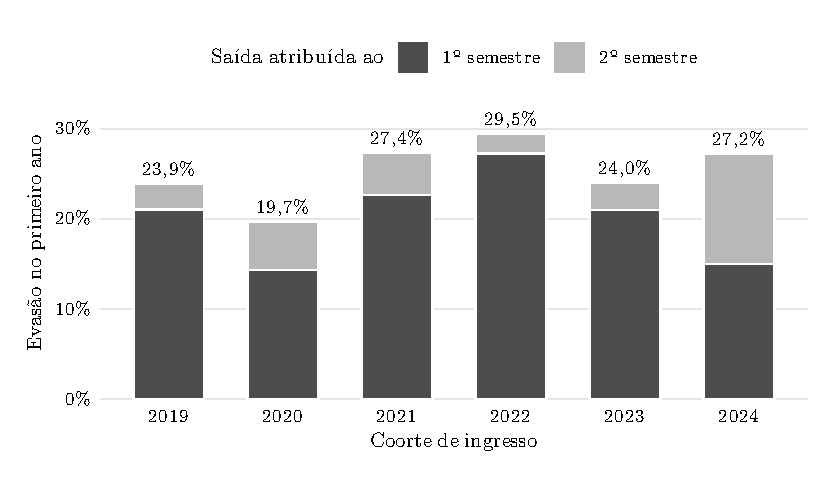
\includegraphics[width=0.85\textwidth]{fig_tcc_evasao_coorte.eps}
  \caption{Evasão no primeiro ano por coorte, segundo o semestre a que a saída foi atribuída, em percentual dos ingressantes de cada coorte ($N = 1{.}320$). O número sobre cada barra é a taxa do primeiro ano.}
  \label{fig:coorte}
\end{figure}

Entre os cursos, a evasão no primeiro ano foi de 21,1\%, na licenciatura em Química, a 27,4\%, no bacharelado em Física (Tabela~\ref{tab:curso}). Todos os intervalos incluíram a taxa geral (Figura~\ref{fig:categorias}). Em todos, a maior parte das saídas foi atribuída ao primeiro semestre, de 75\% das evasões, na licenciatura em Física, a 88\%, em Estatística. O perfil de ingresso também variou pouco, pois a parcela com renda familiar de até 1 SM foi de 8,2\% a 15,2\%, a de cotistas, de 43,8\% a 52,6\% e a nota total mediana, de 623 a 663 pontos, em uma escala em que os pesos das provas mudam de um curso a outro.

\begin{table}[H]
  \centering
  \caption{Evasão no primeiro ano e perfil de ingresso por curso ($N = 1{.}320$). As saídas no 1º semestre estão em percentual das evasões do curso e a renda, entre os que a informaram. A nota total é a do Sisu, com os pesos das provas de cada curso.}
  \label{tab:curso}
  \tabela{tab_tcc_curso.tex}
\end{table}

\begin{figure}[H]
  \centering
  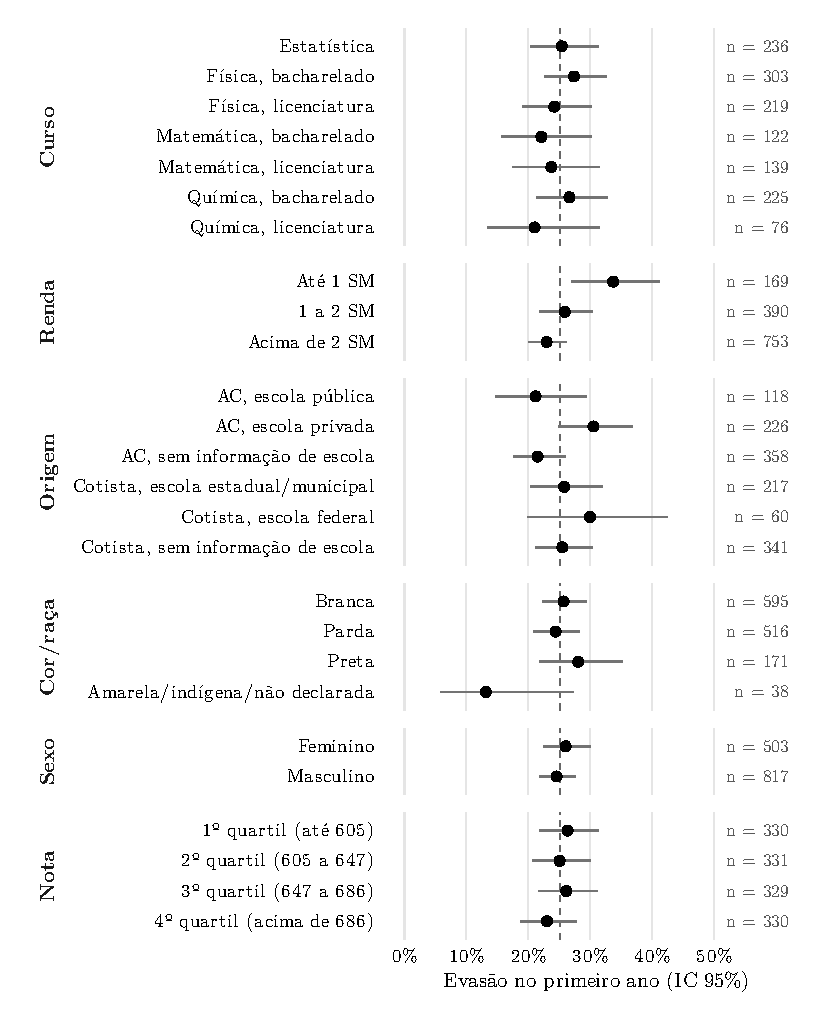
\includegraphics[width=0.85\textwidth]{fig_tcc_evasao_categorias.eps}
  \caption{Evasão no primeiro ano segundo características de ingresso, com intervalo de confiança (IC) de 95\% de \citet{wilson1927probable}, sem ajuste pelas demais características ($N = 1{.}320$; na renda, as 1.312 matrículas com a informação). A linha tracejada marca a taxa geral (25,2\%) e $n$ é o número de ingressantes da categoria. AC indica ampla concorrência.}
  \label{fig:categorias}
\end{figure}

No histórico do primeiro semestre, as disciplinas com mais registros foram introdutórias de matemática, como Cálculo I, Geometria Analítica e Matemática Básica I; e da área de cada curso, como Física I, Química Geral I e Estatística I. Nesse semestre, a reprovação foi comum também entre quem permaneceu. Nas coortes de calendário regular, a grande maioria deles reprovou em pelo menos uma disciplina (76\%; Tabela~\ref{tab:reprovacao}). A reprovação por nota foi até mais frequente entre eles do que entre os que saíram no primeiro semestre (66\% contra 48\%). Já a reprovação por frequência foi mais comum entre os que saíram (56\% contra 36\%). Para os que saíram no segundo semestre, os únicos em que a reprovação do primeiro antecede a saída, a reprovação por frequência foi mais comum do que entre os que permaneceram (48\% contra 36\%), mas o grupo tem só 29 estudantes. Dos 93 ingressantes que trancaram a matrícula no primeiro ano sem sair, a maioria deixou o curso nos anos seguintes, em proporção bem maior que a dos demais que permaneceram (77\% contra 47\%, com seguimento até 2025; Tabela~\ref{tab:trancamento}).

Uma parte das saídas do primeiro semestre foi lançada ainda durante o semestre. A maioria delas não deixou nenhum registro no histórico. Nas coortes de calendário regular, ficaram sem registro 72\% das saídas do primeiro semestre lançadas até junho, contra 17\% das lançadas depois. Fora a coorte de 2020, esse tipo de saída foi mais comum entre os cotistas de escola estadual ou municipal (11,4\% dos ingressantes) e menos comum na ampla concorrência vinda de escola pública (4,9\%).

Nas taxas brutas, a diferença mais visível entre as categorias apareceu na renda (Figura~\ref{fig:categorias}; os valores estão na Tabela~\ref{tab:descritiva}, no Apêndice~\ref{apendice:reprovacao}). Um terço dos estudantes com renda familiar de até 1 SM evadiu (33,7\%), contra cerca de um quarto nas faixas superiores. Como o estrato reúne só um em cada oito ingressantes, qualquer comparação que o envolva tem precisão limitada. Na ampla concorrência, quem veio de escola privada evadiu mais do que quem veio de escola pública (30,5\% contra 21,2\%). Entre os cotistas, a taxa ficou próxima da média. A exceção foram os cotistas de escola federal, que evadiram tanto quanto a ampla concorrência de escola privada (30,0\%), em um grupo de apenas 60 ingressantes. As diferenças por cor/raça foram pequenas. Pela nota total do Sisu, a evasão quase não mudou do primeiro ao terceiro quartil e foi um pouco menor no quarto (23,0\%, contra 26,4\% no primeiro). Os ingressantes de até 18 anos evadiram mais do que os de 19 e 20 anos (27,9\% contra 21,0\%) e os de 21 anos ou mais ficaram perto destes.

A renda familiar acompanhou a origem, pois a renda mediana dos cotistas, em cada categoria, ficou abaixo da de todas as categorias da ampla concorrência (Tabela~\ref{tab:renda-origem}). Todas as categorias da origem, porém, reuniram estudantes das três faixas. Mais de um terço dos cotistas de escola estadual ou municipal e dos cotistas sem informação de escola tinha renda acima de 2 SM. Mais da metade dos cotistas ingressou por vagas reservadas sem critério de renda (338 de 611), com renda mediana entre a das vagas com esse critério e a da ampla concorrência. O limite de 1,5 SM per capita, critério das cotas até 2023, abrangeu também dois terços da ampla concorrência (67,8\%).

\begin{table}[H]
  \centering
  \caption{Renda familiar segundo a origem e a modalidade de ingresso, nas
  matrículas com renda informada ($n = 1{.}312$). A última coluna traz a renda
  familiar per capita de até 1,5 SM, critério de renda das cotas até 2023.
  AC indica ampla concorrência.}
  \label{tab:renda-origem}
  \setlength{\tabcolsep}{3pt}
  \tabela{tab_art_renda_origem.tex}
\end{table}

Quanto ao perfil de entrada, o CCE recebe um público semelhante ao do restante da Ufes. Entre os ingressantes do primeiro semestre de 2018 a 2024 que responderam à questão de renda, a parcela com renda familiar de até 1 SM é parecida no Centro e nos demais cursos (12,1\% e 13,6\%). Por incluir a coorte de 2018, essa parcela do CCE difere da das matrículas analisadas (12,9\%). A parcela de cotistas também é parecida (47,0\% e 47,5\%), assim como a de estudantes pretos, pardos e indígenas (53,4\% e 51,4\%). Ao fim do primeiro ano, a composição por modalidade praticamente não mudou, porque cotistas e não cotistas foram retidos em proporções próximas (Tabela~\ref{tab:composicao}). A perda concentrou-se no estrato de renda mais baixa, do qual dois terços permaneceram (66,3\%) e, em menor grau, entre os estudantes pretos. Como esses grupos são pequenos, sua participação no corpo discente caiu pouco (1,5 ponto percentual no estrato de renda e 0,6 entre os pretos).

\begin{table}[H]
  \centering
  \caption{Composição do corpo discente no ingresso e após o primeiro ano, e
  retenção no primeiro ano. Percentuais calculados entre os ingressantes com a
  informação disponível.}
  \label{tab:composicao}
  \tabela{tab_art_composicao.tex}
\end{table}

\subsubsection{Associações com a evasão}
\label{sec:res-modelo}

No modelo ajustado, a renda teve indício fraco de associação à evasão (teste global, p = 0,079; Tabela~\ref{tab:modelo}). A curva estimada cai das rendas mais baixas até cerca de 3 SM e fica quase plana depois (Figura~\ref{fig:renda}). Com renda familiar de 1 SM, o risco estimado foi cerca de um quarto maior que o da renda mediana, de 2,25 SM (RR 1,27; 1,04–1,54). Com 5 SM, ficou próximo do da mediana. O intervalo de cada ponto vale só para aquele ponto e se alarga nas pontas da escala. Por isso, a leitura da curva inteira vem do teste global. As estimativas das demais covariáveis, com os seus intervalos, estão na Figura~\ref{fig:floresta}. A nota total do Sisu, pela qual o estudante foi classificado, não se associou à evasão de forma distinguível (RR 0,92 por 100 pontos; 0,77–1,10). Nas verificações da forma da nota, a interação com o curso (p = 0,61) e o desvio da linearidade (p = 0,24) não se distinguiram. A nota padronizada dentro de cada curso e coorte também não se distinguiu (RR 0,97 por desvio-padrão; 0,87–1,08).

\begin{table}[H]
  \centering
  \caption{Risco relativo de evasão no primeiro ano no modelo principal
  (Poisson modificado, variância robusta HC3; $n = 1{.}312$; 331 eventos). Na renda, RR em relação à mediana em três pontos da curva e valor $p$ do teste global. Nas categorias, o $p$ de cada contraste com a referência aparece por ser usual; a leitura de cada variável vem do teste global. A referência da origem é a do estudo nacional com que os resultados se comparam \citep{paulaDESIGUALDADESAPOSACESSO2024}. IC indica intervalo de confiança; gl, graus de liberdade; e AC,
  ampla concorrência.}
  \label{tab:modelo}
  \tabela{tab_art_modelo.tex}
\end{table}

\begin{figure}[H]
  \centering
  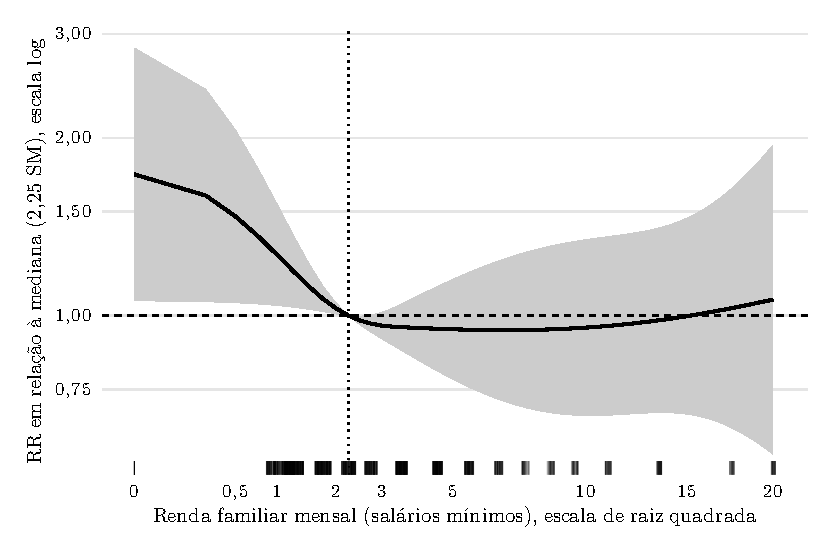
\includegraphics[width=0.85\textwidth]{fig_art_renda_curva.eps}
  \caption{Risco relativo de evasão no primeiro ano segundo a renda familiar, em
  relação à renda mediana (2,25 SM), no modelo principal. A linha vertical pontilhada marca a mediana, ponto de referência em que o RR vale 1 por construção. A faixa cinza é o IC 95\% de cada ponto da curva, sem ajuste para a curva inteira, cuja associação com a evasão é avaliada pelo teste global (Tabela~\ref{tab:modelo}).
  As marcas no eixo horizontal são os valores observados, com pequeno deslocamento
  aleatório. Acima de 10 SM há poucos dados. O eixo horizontal está em escala de raiz quadrada, que abre o trecho das rendas mais baixas.}
  \label{fig:renda}
\end{figure}

\begin{figure}[H]
  \centering
  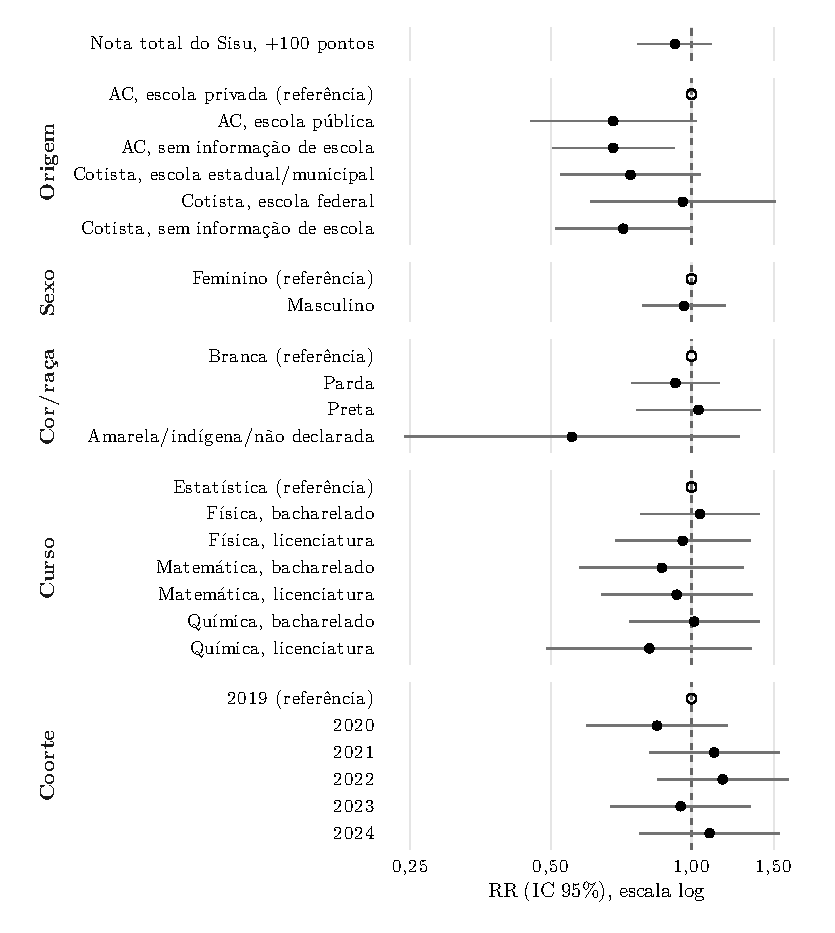
\includegraphics[width=0.85\textwidth]{fig_tcc_rr_floresta.eps}
  \caption{Risco relativo de evasão no primeiro ano no modelo principal, com IC 95\%, para as covariáveis além da renda (Figura~\ref{fig:renda}). Na nota, o RR se refere a um acréscimo de 100 pontos e, nas categorias, à referência indicada em cada grupo. Os valores estão na Tabela~\ref{tab:modelo} e, para curso e coorte, na Tabela~\ref{tab:logbin}. AC indica ampla concorrência.}
  \label{fig:floresta}
\end{figure}

Como a nota, a origem não se distinguiu (teste global, p = 0,12). Em relação à ampla concorrência de escola privada, as estimativas das demais categorias ficaram abaixo de 1, entre 0,68 e 0,74. Os cotistas de escola federal, grupo pequeno e de intervalo mais largo, tiveram estimativa próxima de 1 (RR 0,96; 0,61–1,51). Comparados diretamente a cada uma das outras quatro categorias, tiveram RR entre 1,29 e 1,41. Os quatro intervalos dessas comparações incluíram 1, com limites inferiores de 0,81 a 0,90 e superiores de 2,06 a 2,41. A correlação com as demais covariáveis, a renda entre elas, pouco pesou na largura dos intervalos da origem e da renda, visto que, pelo GVIF, aumentou os seus erros-padrão em cerca de 7\% e 6\% (Tabela~\ref{tab:gvif}). A nota foi o termo mais afetado, com erro-padrão cerca de 29\% maior do que teria sem correlação com as demais covariáveis. O sexo (RR 0,96; 0,79–1,18) e a cor/raça (teste global, p = 0,45) também não se distinguiram, nem os sete cursos (p = 0,93).

No diagnóstico, o ajuste convergiu e todos os riscos preditos ficaram abaixo de 1. Retiradas as dez matrículas de maior distância de Cook, o teste da renda passou de p = 0,079 para p = 0,11. Nenhuma matrícula, ao ser retirada, moveu a estimativa da renda em 1 SM nem a da nota em mais de 0,22 erro-padrão. Na forma da média, o teste da ligação indicou desvio (p = 0,046), que a troca pela ligação logit não removeu. A soma de quadrados dos resíduos ficou próxima da esperada sob o modelo (p = 0,48) e os resíduos parciais acompanharam a curva da renda e a reta da nota (Apêndice~\ref{apendice:comparacao}). Com a variância agrupada por pessoa, nem os testes da renda e da origem nem o ganho de discriminação mudaram de leitura. Com as formas HC0, HC1 e HC2 no lugar da HC3, os erros-padrão ficaram no máximo 4,5\% menores e os testes da renda e da origem mantiveram a leitura.

Nas quinze análises de sensibilidade (Figura~\ref{fig:sensibilidade}; valores na Tabela~\ref{tab:sensibilidade}, no Apêndice~\ref{apendice:comparacao}), o indício da renda se mostrou frágil. O indício se manteve sem a coorte de 2020, sem a nota total e com a imputação da renda ausente. Com a escolaridade da mãe e a idade no modelo, o teste ficou abaixo de 0,05. A diferença veio das 30 matrículas sem essas informações, não das covariáveis acrescentadas, pois nessas mesmas matrículas, sem elas, o teste também ficava abaixo de 0,05 (Apêndice~\ref{apendice:mae-idade}). Nas outras onze análises, a evidência ficou mais fraca, com valores p acima de 0,10. Entre elas estão todas as que retiram a coorte de 2024 e as duas que trocam só o estimador, o log-binomial e a regressão logística. Fora dessas análises, quando a faixa de até 1 SM recebeu o seu ponto médio, de 0,5 SM, o teste ficou na fronteira de 0,05 (Apêndice~\ref{apendice:comparacao}).

A origem não se distinguiu em quase todas as variantes. A exceção foi a janela de dois anos, em que ela se associou à evasão (p = 0,024). Nessa janela, as estimativas mais baixas em relação à ampla concorrência de escola privada foram as da ampla concorrência de escola pública e das duas categorias sem informação de escola. Com o trancamento contado como evento, a nota total se associou a menor risco (RR 0,82; 0,71–0,96). Nessa variante, a origem teve indício fraco.

\begin{figure}[H]
  \centering
  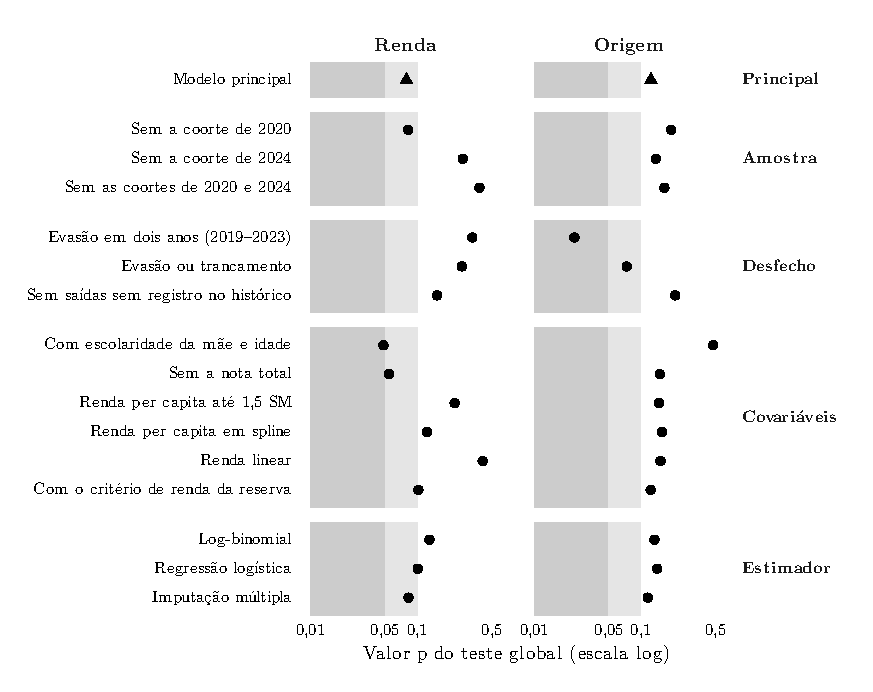
\includegraphics[width=0.9\textwidth]{fig_tcc_sensibilidade.eps}
  \caption{Valor $p$ do teste global da renda e da origem no modelo principal (triângulo) e em cada análise de sensibilidade, em escala log. A faixa escura marca $p$ abaixo de 0,05 e a clara, de 0,05 a 0,10. Os valores estão na Tabela~\ref{tab:sensibilidade} (Apêndice~\ref{apendice:comparacao}).}
  \label{fig:sensibilidade}
\end{figure}

Na variante que acrescenta a escolaridade da mãe e a faixa etária, a idade se associou à evasão (p = 0,043). Os ingressantes de 19 e 20 anos e os de 21 anos ou mais tiveram risco estimado menor do que os de até 18 (Tabela~\ref{tab:mae-idade}). A escolaridade da mãe não se distinguiu (p = 0,59). Com a idade no modelo, as duas categorias de origem sem informação de escola, onde se concentram os mais velhos, ficaram mais perto da ampla concorrência de escola privada do que no modelo principal com as mesmas matrículas. O teste da origem deu p = 0,48.

Das variantes, a que retira a coorte de 2024 pede uma leitura à parte, porque retirar só a de 2020 quase não mudou o teste (p = 0,083). A coorte de 2024, cuja retirada leva 49 das 331 evasões, teve o calendário alterado pela greve e nela a admissão seguiu pela primeira vez a nova regra de cotas. Nas coortes de calendário regular, os estudantes com renda de até 1 SM evadiram mais do que os com renda acima de 2 SM, como nas de calendário alterado, onde a diferença foi maior (Tabela~\ref{tab:renda-coortes}). Nas regulares, o intervalo incluiu 1 (RR 1,34; 0,94–1,90). O termo de interação não distinguiu os dois grupos de coortes, nem com a renda nessas faixas (p = 0,10) nem em \textit{spline} (p = 0,47).

\begin{table}[H]
  \centering
  \caption{Evasão segundo a renda familiar em coortes de calendário regular e alterado, com o RR
  da renda de até 1 SM em relação a mais de 2 SM (modelo com renda em faixas).
  No teste da interação entre renda e tipo de coorte, $p = 0{,}10$ com a renda em faixas e
  $p = 0{,}47$ em \textit{spline}.}
  \label{tab:renda-coortes}
  \tabela{tab_art_renda_coortes.tex}
\end{table}

\subsubsection{Discriminação}
\label{sec:res-discriminacao}

A AUC corrigida da linha de base com curso e coorte foi de 0,518 (Figura~\ref{fig:discriminacao}; valores na Tabela~\ref{tab:auc}, no Apêndice~\ref{apendice:comparacao}), próxima do valor de 0,5 que corresponde a discriminação nula, de modo que a discriminação dos modelos seguintes vem, na prática, só das características de ingresso. Na Figura~\ref{fig:discriminacao}, as curvas ROC da linha de base e do modelo completo ficam próximas da diagonal. A mesma figura traz a AUC corrigida de cada modelo com o seu intervalo. Acrescentado sozinho, cada bloco de informações de ingresso somou no máximo 0,015 à AUC corrigida. Com todos os blocos juntos, o teste conjunto não distinguiu de zero os coeficientes acrescentados (p = 0,12). O ganho estimado do modelo completo sobre a linha de base foi de 0,023 ($-$0,011 a 0,055). Mesmo a AUC aparente, calculada nos dados do próprio ajuste e por isso otimista, foi de 0,598. Em termos práticos, dado um estudante que evadiu e outro que permaneceu, o modelo atribui maior risco ao primeiro em pouco mais da metade dos pares e, no limite superior do intervalo da AUC corrigida (0,576), ainda em menos de 60\% deles. Em uma simulação, esse intervalo, adaptado para este estudo, cobriu a AUC verdadeira em 85\% das amostras, abaixo dos 95\% nominais. Quando errou, ficou quase sempre acima dela, de modo que o limite superior tende a exagerar a discriminação (Apêndice~\ref{apendice:comparacao}).

\begin{figure}[H]
  \centering
  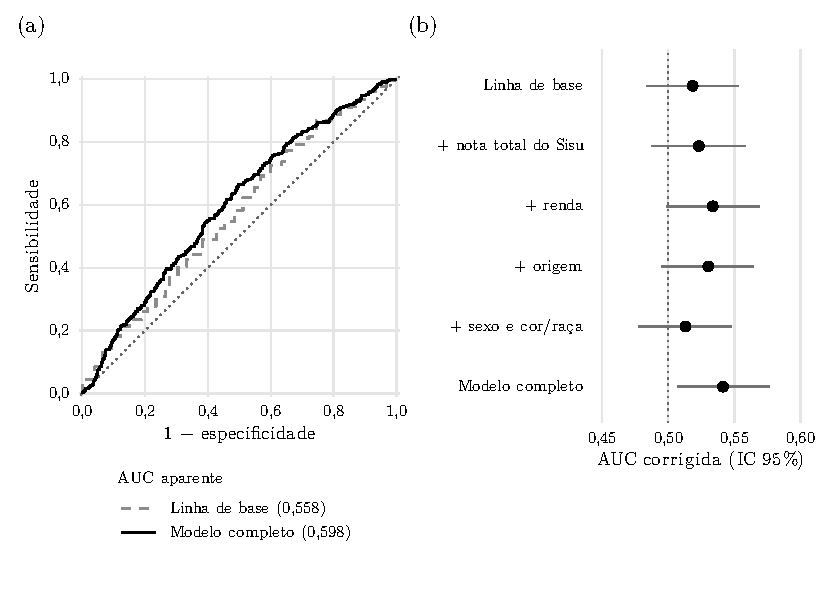
\includegraphics[width=0.85\textwidth]{fig_tcc_discriminacao.eps}
  \caption{Discriminação dos modelos. (a) Curvas ROC da linha de base (curso e coorte) e do modelo completo, calculadas nos dados do próprio ajuste, com a AUC aparente na legenda; a diagonal pontilhada corresponde a um modelo que não discrimina. (b) AUC corrigida por otimismo, com IC 95\% por \textit{bootstrap}, da linha de base, da linha de base acrescida de cada bloco e do modelo completo. Em uma simulação, os intervalos da AUC corrigida e do $\Delta$AUC cobriram o valor-alvo em 85\% e 91\% das amostras (Apêndice~\ref{apendice:comparacao}).}
  \label{fig:discriminacao}
\end{figure}

\subsubsection{Análises complementares}
\label{sec:res-complementar}

Com a renda em faixas, a renda se associou à evasão (teste global, p = 0,030), em um corte em 1 SM que veio da exploração inicial dos dados. O risco dos estudantes com renda familiar de até 1 SM foi quase 50\% maior do que o dos estudantes com mais de 2 SM (RR 1,47; 1,10–1,95). A faixa intermediária não se distinguiu da superior (Tabela~\ref{tab:complementar}). Já a nota de uma única área, cada uma em modelo próprio no lugar da nota total, associou-se a menor risco, tanto em CN quanto em MT, com AUC corrigida ligeiramente maior. As duas notas têm correlação de Pearson de 0,52.

\begin{table}[H]
  \centering
  \caption{Análises complementares: renda em faixas no lugar do \textit{spline}
  e nota de uma área no lugar da nota total, mantidas as demais covariáveis do
  modelo principal. AUC corrigida por otimismo.}
  \label{tab:complementar}
  \tabela{tab_art_complementar.tex}
\end{table}

Nas interações exploratórias com o curso, a renda teve indício fraco de associação diferente entre os cursos, tanto em faixas (p = 0,061) quanto pela faixa de até 1 SM (p = 0,073). A interação do curso com ser cotista não se distinguiu (p = 0,76). O RR da faixa de até 1 SM em relação às rendas acima foi maior nas três licenciaturas e no bacharelado em Estatística (de 1,50 a 2,61) e ficou perto de 1 ou abaixo nos bacharelados em Física, Matemática e Química (de 0,74 a 0,93; Figura~\ref{fig:renda-curso}). Em cada curso, porém, essa faixa reuniu de 2 a 12 evasões. Nos cursos menores, os intervalos vão de 0,21 a 6,69. Esses testes têm pouco poder, porque cada curso teve de 16 a 83 evasões.

\begin{figure}[H]
  \centering
  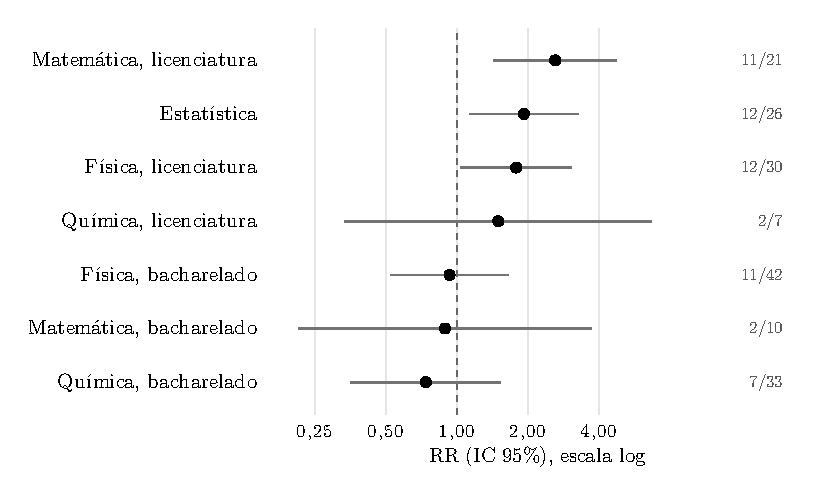
\includegraphics[width=0.85\textwidth]{fig_tcc_renda_curso.eps}
  \caption{RR de evasão no primeiro ano da renda familiar de até 1 SM em relação às rendas acima, em cada curso, no modelo principal com a renda trocada pela faixa de até 1 SM e a interação dessa faixa com o curso (exploratório; $n = 1{.}312$). À direita, evasões e ingressantes na faixa de até 1 SM. Os valores estão na Tabela~\ref{tab:renda-curso}.}
  \label{fig:renda-curso}
\end{figure}

\subsection{Discussão}
\label{sec:discussao}

\subsubsection{Renda, origem e demais características de ingresso}
\label{sec:disc-renda-origem}

Ajustadas uma pela outra, a renda manteve um indício fraco de associação com a evasão, enquanto a origem não se distinguiu. Indício fraco, com p entre 0,05 e 0,10, quer dizer que os dados são pouco compatíveis com a ausência de associação, mas não o bastante para afirmá-la. Não se pode dizer, assim, qual das duas permanece associada quando a outra é levada em conta, porque a evidência sobre a renda fica ainda mais fraca sem a coorte de 2024 e com a troca do estimador. Os intervalos da origem, por sua vez, são largos.

A fraqueza do indício é a que se esperaria se os admitidos de renda baixa fossem mais selecionados do que os de renda alta em características não medidas, como habilidades e aspirações, que também favorecem a permanência. É o argumento da seleção na entrada \citep{mare1980social}, que estes dados não permitem testar.

Que a evidência fique mais fraca sem a coorte de 2024 admite leituras entre as quais os dados não decidem, porque o teste de interação não distinguiu as coortes de calendário alterado das de calendário regular e retirar uma coorte inteira reduz a precisão. Pela primeira leitura, a associação com a renda se acentuaria na greve de 2024, já que retirar só a coorte de 2020, a do ensino remoto, manteve o indício. Pela segunda, teria intensidade parecida em todas as coortes e só foi estimada com menos precisão nos grupos menores. Pela terceira, a faixa de até 1 SM, que nas coortes de 2019 e 2020 reunia poucos ingressantes, não reúne o mesmo grupo em todas as coortes. O indício refletiria, então, essa mudança do que a faixa reúne. A coorte de 2024 foi ainda a primeira admitida pela nova regra de cotas e a de maior parcela de ingressantes com renda de até 1 SM. Nela o calendário alterado e a mudança na regra de admissão coincidem. Só mais coortes de calendário regular, admitidas pela regra atual, permitiriam distinguir essas leituras.

Nas interações exploratórias, a associação com a renda pareceu concentrar-se nas três licenciaturas e no bacharelado em Estatística, não nos bacharelados em Física, Matemática e Química. A leitura pede cautela por dois motivos. O primeiro é que tanto os testes quanto esse agrupamento dos cursos vieram depois de vistos os dados. Os testes, além disso, foram vários e deram só indício fraco. O segundo é que a faixa de até 1 SM tem poucas evasões em cada curso, de modo que o contraste se apoia em grupos pequenos. Se o padrão se confirmar em outras coortes, a pergunta passa a ser o que, nesses cursos, faz a renda pesar mais. Estes dados não permitem responder a essa pergunta.

A origem não foi descartada nem confirmada, pois, no modelo principal, os intervalos das suas categorias vão de riscos perto da metade do da ampla concorrência de escola privada a riscos parecidos com esse e, nos cotistas de escola federal, a uma vez e meia esse risco. Das quinze análises de sensibilidade, só a que acompanha por dois anos as coortes de 2019 a 2023 associou a origem à evasão. Outra, com o trancamento contado como evento, deu indício fraco. Ser cotista acompanha renda mais baixa sem defini-la, porque cada categoria da origem reúne estudantes de todas as faixas e mais da metade dos cotistas entrou por vagas sem critério de renda. O limite de renda das cotas alcançava ainda a maioria da ampla concorrência. Por isso as duas variáveis puderam ser estimadas juntas e a correlação entre elas pouco alargou os intervalos, cuja largura vem sobretudo do número de matrículas em cada categoria. Dentro da origem, os cotistas vindos de escola federal tiveram risco estimado próximo ao da ampla concorrência vinda de escola privada. A diferença em relação às demais categorias não se distinguiu.

Na análise de sensibilidade, a escolaridade da mãe não se distinguiu. O intervalo dos filhos de mães com ensino superior inclui tanto risco menor quanto maior. No CCE, portanto, ter mãe com diploma não se mostrou nem proteção nem risco no primeiro ano. Neste desfecho, a informação sobre o sistema de ensino que a família transmite pode ajudar a permanecer no curso e também a trocar de curso, o que conta como evasão \citep{nogueira2002sociologia}. Separar os dois efeitos exigiria conhecer o destino de quem sai.

No mesmo modelo, a idade se associou à evasão, com risco estimado maior entre os ingressantes de até 18 anos. Os mais velhos se concentram nas duas categorias de origem sem informação de escola, que reúnem sobretudo quem concluiu o ensino médio antes do ano do exame, de modo que a idade e a origem dividem a mesma informação. Com a idade no modelo, as estimativas dessas duas categorias se aproximaram da referência (Apêndice~\ref{apendice:mae-idade}). Como nelas estão todos os ingressantes de 21 anos ou mais e a maior parte dos de 19 e 20, a estimativa da idade mede sobretudo a diferença por idade dentro dessas duas categorias.

Sexo e cor/raça, que entraram no modelo sem hipótese própria, também não se distinguiram. Os intervalos comportam diferenças moderadas de risco em qualquer direção, sobretudo nas categorias de cor/raça com poucos ingressantes. Por isso, o resultado não indica que homens e mulheres, ou brancos, pardos e pretos, evadam na mesma proporção. Ao fim do primeiro ano, a composição do corpo discente por cor/raça mudou pouco.

\subsubsection{A nota de seleção}
\label{sec:disc-nota}

Entre as características somadas, a nota pela qual o estudante foi classificado no Sisu não se associou à evasão de forma distinguível nem acrescentou discriminação. A estimativa ficou na direção de menor risco. O intervalo vai de um risco quase um quarto menor a um décimo maior a cada 100 pontos. Os dados comportam, portanto, tanto a ausência de associação quanto uma redução moderada do risco com a nota, sem decidir entre as duas. Parte dessa imprecisão vem do próprio desenho. A comparação se faz dentro de sete cursos e ajustada por eles. Em cada curso e modalidade, a seleção pelo Sisu admite só quem alcança a nota de corte, o que estreita as diferenças de nota entre os admitidos e alarga o intervalo. A correlação da nota com as demais covariáveis também o alarga, mais do que o de qualquer outro termo do modelo.

Quando entraram no lugar da nota total, as notas de Ciências da Natureza e de Matemática, que correspondem ao conteúdo dos cursos, associaram-se cada uma a menor risco. A nota total as combina com linguagens, ciências humanas e redação. Daí a hipótese, tirada de análise complementar, de que o preparo específico se associe mais à permanência do que o desempenho geral. Cada nota entrou em um modelo próprio e, como as duas são correlacionadas, não é possível atribuir a associação a uma ou a outra.

Além do preparo que mede, a nota orienta a escolha do curso, pois, no Sisu, o candidato conhece a própria nota antes de indicar as opções \citep{klitzkeFATORESASSOCIADOSEVASAO2023}. A ordem de opção, um dos elementos do compromisso inicial no modelo de Tinto, não consta do cadastro da Ufes. A nota de seleção talvez reúna dois perfis de estudante, a saber, o que escolheu o curso e o que chegou a ele pela nota.

\subsubsection{Discriminação}
\label{sec:disc-discriminacao}

Somadas ao curso e à coorte, as características registradas no ingresso quase não melhoraram a discriminação entre quem deixou o curso no primeiro ano e quem permaneceu. Tomados ao acaso um estudante que saiu e outro que ficou, o modelo completo atribui maior risco ao que saiu pouco mais vezes do que o faria um sorteio e, mesmo no limite superior do intervalo da AUC corrigida, que tende a exagerá-la, em menos de seis de cada dez pares. A discriminação baixa convive com o indício de associação da renda, porque as duas medidas respondem a perguntas diferentes. Mesmo na faixa de até 1 SM, a de maior evasão, que reúne um em cada oito ingressantes, dois terços permaneceram. Por isso, conhecer a renda pouco ajuda a ordenar quem sai acima de quem fica. O resultado é compatível com o modelo de \citet{tintoDropoutHigherEducation1975}, que situa a decisão de sair depois da matrícula, mas não chega a testá-lo, pois a mesma discriminação baixa apareceria se as variáveis de ingresso fossem medidas com erro ou se a própria seleção pelo Sisu tivesse estreitado as diferenças entre os admitidos.

\subsubsection{O registro da saída}
\label{sec:disc-registro}

A maior parte das saídas do primeiro ano foi atribuída ao primeiro semestre e lançada no fim do período letivo ou no intervalo entre semestres. O que os dados mostram, portanto, é a não renovação da matrícula, não a data em que o estudante decidiu sair, que pode ter sido semanas antes. Uma parte menor foi lançada ainda durante o semestre. Essas saídas, na maioria, não deixaram nenhum registro no histórico. O histórico não diz se esses estudantes chegaram a cursar. É possível que parte deles tenha trocado de opção logo após a matrícula.

Para quem saiu no primeiro semestre, a reprovação e a saída aparecem nos registros ao mesmo tempo, ao fim do período letivo, sem que se saiba qual veio antes. A reprovação por frequência foi mais comum entre esses estudantes porque é, em boa parte, o registro do próprio abandono, já que quem deixa de frequentar as aulas é reprovado por falta nas disciplinas em que continuava matriculado. Já a reprovação por nota foi mais comum entre os que permaneceram, em parte porque quem abandona tende a ser reprovado por falta e a maioria dos que ficaram reprovou em alguma disciplina. A dificuldade das disciplinas introdutórias é, assim, compartilhada por quem fica e por quem sai. Entre os que saíram no segundo semestre, os únicos em que a reprovação do primeiro antecede a saída, a reprovação por frequência foi mais comum. O grupo é pequeno e a falta pode registrar um abandono já começado no primeiro semestre. Se a decisão de sair se forma nas primeiras semanas, um sinal que só aparece no histórico ao fim do semestre chega depois dela.

Ao contrário da reprovação, o trancamento é registrado no momento em que ocorre. A maioria dos que trancaram a matrícula no primeiro ano sem sair deixou o curso nos anos seguintes, bem mais do que os demais estudantes que permaneceram, o que sugere que trancar seja, muitas vezes, uma evasão adiada. Contado como permanência, como no indicador do Inep, o trancamento deixa parte das evasões tardias no grupo de referência.

\subsubsection{Limitações}
\label{sec:disc-limitacoes}

A direção do viés muda de uma limitação para outra e só para algumas ela é conhecida. A renda vem de uma declaração em faixas, convertida em um valor por faixa, quase sempre o ponto médio. Esse erro reduz a precisão e a discriminação possível. Como a renda se correlaciona com a origem, a estimativa de cada uma pode se deslocar para mais ou para menos \citep{keogh2020stratos}. Ao contrário do teste da renda, o da origem não tem, por isso, validade garantida. A faixa de até 1 SM, além disso, não reúne o mesmo grupo em todas as coortes, pois, nas de 2019 e 2020, poucos ingressantes declararam essa renda (Tabela~\ref{tab:coorte}).

Em cada curso e modalidade, a seleção pelo Sisu admite só quem alcança a nota de corte e, ao estreitar as diferenças de nota entre os admitidos, alarga o intervalo da nota e reduz a discriminação, sem deslocar o risco relativo enquanto a admissão depender só de variáveis do modelo. Se dependeu também de características não observadas ligadas à evasão, o deslocamento é possível em qualquer sentido.

Na especificação, o teste da ligação indicou algum desvio na média do modelo principal, que a troca da ligação não removeu e que os resíduos não localizaram (Apêndice~\ref{apendice:comparacao}). Pelo sinal do desvio, o modelo exagera o risco das matrículas de maior risco predito. Nesse caso, os RR das categorias de maior risco, como a renda mais baixa, estariam um pouco acima dos verdadeiros, embora o RR em 1 SM tenha sido o mesmo com a ligação logit.

No registro do Inep, a escola de origem só é conhecida para quem concluiu o ensino médio no ano do exame. Assim, cerca de metade dos ingressantes ficou nas categorias sem essa informação. As estimativas das categorias com informação valem para esse subgrupo.

No registro da Ufes, o grupo de referência inclui os trancados e as saídas não lançadas até a extração dos dados. Se o sub-registro das saídas atingir todos os grupos na mesma proporção e nenhuma saída tiver sido lançada indevidamente, as taxas de evasão ficam subestimadas, mas os riscos relativos se mantêm. Se atingir uns grupos mais do que outros, o grupo com mais sub-registro parece evadir menos do que de fato evade. A sensibilidade com o trancamento contado como evento mostra que o deslocamento não é o mesmo para todas as variáveis. Nela, a evidência sobre a renda ficou mais fraca, enquanto a nota total passou a se associar a menor risco. O desfecho reúne ainda dois tipos de saída, a não renovação ao fim do semestre e a desistência lançada durante ele, que pode incluir quem não chegou a cursar e que nenhuma forma de saída distingue, já que todas foram lançadas como desistência. Retiradas essas desistências, nem a renda nem a origem se distinguiram (Tabela~\ref{tab:sensibilidade}).

Faltam aos dados informações que a literatura associa à permanência, como a assistência estudantil, o trabalho, a frequência nas primeiras semanas e a ordem de opção no Sisu. No modelo de \citet[pp.~585, 589]{cabrera1992role}, por exemplo, ter recebido ajuda financeira age sobre a integração social e as notas do estudante. Se a assistência estudantil, dirigida aos estudantes de menor renda, acompanha maior permanência, a associação observada com a renda é a que existe com esse apoio em vigor, provavelmente menor do que seria sem ele. Sem a trajetória acadêmica no modelo, o estudo não compara o peso do ingresso com o da trajetória.

O alcance é o de uma instituição, pois os resultados vêm de sete cursos de quatro áreas em uma única universidade, em seis coortes, duas delas de calendário alterado, pelo ensino remoto e pela greve. O estudo, por fim, não avalia nenhuma política de permanência. O indício de associação com a renda aponta em que grupo a evasão precoce tende a ser mais frequente, sem permitir identificar quem vai sair.

% ==============================================================================
% VII. CONCLUSÃO
% ==============================================================================
\section{Conclusão}
\label{sec:conclusao}

Este estudo examinou, nos sete cursos do Centro de Ciências Exatas da Ufes, se as características registradas no ingresso pelo Sisu se associam à evasão no primeiro ano e quanto ajudam a distinguir quem sai de quem permanece. Dos ingressantes de 2019 a 2024, um quarto deixou o curso no primeiro ano. A troca de curso contou como evasão, como nos indicadores do Inep, porque o registro da Ufes informa a saída do curso de ingresso, sem o destino de quem sai. A maior parte dessas saídas foi atribuída ao primeiro semestre e lançada no fim do período letivo ou no intervalo entre semestres. O desfecho é, portanto, a não renovação da matrícula, não o momento em que o estudante decidiu sair, que os registros não guardam.

Das características de ingresso, a renda familiar teve indício fraco de associação com a evasão, com risco estimado maior nas rendas mais baixas, mesmo ajustada pela origem. A curva do risco cai das rendas mais baixas até perto de 3 SM e fica quase plana depois. Em 1 SM, o risco ficou pouco mais de um quarto acima do estimado na renda mediana, de 2,25 SM. Esse indício deve ser tratado como hipótese, porque o modo de incluir a renda no modelo e a leitura dos valores p foram definidos depois de explorados estes mesmos dados. Trata-se também de um achado frágil. Sem a coorte de 2024, que teve o calendário alterado pela greve e foi a primeira admitida pela nova regra de cotas, a evidência ficou ainda mais fraca, como também ficou com outros métodos de estimação. A associação nas coortes de calendário alterado, porém, não se distinguiu da observada nas de calendário regular. Só mais coortes dirão se a de 2024 teve algo de próprio.

Para a nota de seleção, a origem, o sexo e a cor/raça, os dados não permitem afirmar nem descartar associação. Entre a renda e a origem, portanto, não se pode dizer qual permanece associada quando a outra é levada em conta. A dúvida vem da pouca precisão, não da sobreposição entre as duas variáveis, pois ser cotista acompanha renda mais baixa sem defini-la. Mais da metade dos cotistas entrou por vagas sem critério de renda. Por isso, a correlação entre as duas pouco alargou os intervalos da origem, cuja largura vem sobretudo do número de matrículas em cada categoria. Mesmo sem permitir afirmar nem descartar essas associações, os dados mostram até onde elas poderiam ir. Em relação aos estudantes de ampla concorrência vindos de escola privada, o risco de evasão dos demais grupos de origem ficaria entre cerca de metade e uma vez e meia o risco desses estudantes, este último valor só nos cotistas vindos de escola federal. Nenhum grupo, portanto, chegaria ao dobro do risco. Já a cada 100 pontos a mais na nota de seleção, o risco cairia no máximo quase um quarto e subiria no máximo um décimo.

Para distinguir quem sai de quem fica, as características de ingresso serviram pouco. O curso e a coorte, sozinhos, praticamente não separaram os dois grupos. Renda, origem, nota de seleção, sexo e cor/raça, somadas a eles, quase não melhoraram a discriminação. Dados um estudante que saiu e outro que ficou, o modelo atribui maior risco ao que saiu pouco mais vezes do que o faria um sorteio. Mesmo nos dados do próprio ajuste, que a exageram, a discriminação não chegou a 60\% dos pares. No momento da matrícula, portanto, o perfil de ingresso pouco antecipa a evasão precoce nesses cursos.

Os sete cursos se pareceram mais do que se diferenciaram. A evasão no primeiro ano foi de 21,1\%, na licenciatura em Química, a 27,4\%, no bacharelado em Física. Em todos, a maior parte das saídas foi atribuída ao primeiro semestre, com o maior peso em Estatística, onde quase nove em cada dez saídas ocorreram nesse semestre. O perfil de ingresso, em renda, cotas e nota, variou pouco de um curso a outro. Depois do ajuste pelas características de ingresso, o curso não se distinguiu. A licenciatura, que teve mais evasão do que o bacharelado em estudos nacionais e na UFFS, não se separou dele no CCE. Os dados não dizem com segurança se a renda e a origem pesam do mesmo modo em todos os cursos. Nas interações exploratórias, a renda pareceu pesar mais nas três licenciaturas e no bacharelado em Estatística, sobretudo na licenciatura em Matemática, do que nos bacharelados em Física, Matemática e Química, em que o RR da faixa de até 1 SM ficou perto de 1 ou abaixo. O padrão se lê como hipótese, porque os testes vieram depois de vistos os dados e cada curso teve poucas evasões.

Pelo indicador de trajetória do Inep, os cursos do Centro perderam no ano de ingresso 12,0\% dos ingressantes de 2019, perto dos 12,5\% dessas áreas no conjunto das federais \citep{inep2025trajetoria}. O registro da própria Ufes, porém, dá o dobro de saídas para a mesma coorte, taxa que, pelo indicador, esses cursos só ultrapassam no terceiro ano. A diferença não vem de atraso no lançamento, já que todas as saídas do primeiro ano dessa coorte foram lançadas em 2019. Só uma parte dela se explica com estes dados, pelas desistências lançadas no primeiro semestre sem nenhum registro no histórico, que talvez nem tenham chegado ao Censo da Educação Superior como ingressantes. O restante depende do vínculo que cada instituição informa ao Censo, informação a que não se teve acesso. Por isso, as taxas do Inep e as dos registros internos não se comparam diretamente. A semelhança entre o CCE e o conjunto das federais vale dentro do indicador do Inep.

Comparados aos de outras universidades federais, os resultados concordam em parte. Os estudos preditivos de \citet{felizardoAnaliseDiscriminanteProbabilidade2023} e de \citet{salaberriMineracaoDadosEducacionais2024} chegaram a um ponto parecido pelo lado da trajetória, pois as disciplinas cursadas e reprovadas pesaram mais do que as notas de ingresso. A comparação tem limite, porque aqueles estudos medem acurácia de classificação, em outras populações e com outros desfechos, não o ganho sobre um modelo de referência. Na UFFS, os ingressantes com notas do Enem mais altas evadiram menos ao longo de seis anos \citep{nierotkaFatoresAssociadosEvasao2023} e, na UFRJ, a vantagem dos estudantes de nota mais alta só apareceu depois do primeiro ano, em um modelo que inclui o desempenho no curso \citep{klitzkeFATORESASSOCIADOSEVASAO2023}. O intervalo da nota no CCE comporta associações como essas, que talvez precisem de mais de um ano para aparecer.

No estudo nacional de \citet{paulaDESIGUALDADESAPOSACESSO2024}, a chance de deixar o ensino superior cresceu a cada faixa de renda mais baixa, direção que o indício do CCE acompanha, embora lá o desfecho fosse mais restrito, a saída do sistema, que não conta a troca de curso. Nas instituições federais, as probabilidades preditas de abandono dos estudantes mais pobres e dos mais ricos tiveram intervalos que se sobrepuseram, o que não permitiu distingui-las. Para os autores, a seleção por exames concorridos tornaria as desigualdades na evasão menores nas universidades federais e estaduais \citep[p.~14]{paulaDESIGUALDADESAPOSACESSO2024}. O CCE admite pelo Sisu só quem alcança a nota de corte. A fraqueza do indício da renda é, assim, a que esse argumento prevê, embora estes dados não permitam testá-lo. No mesmo estudo, os egressos de escola pública federal tiveram chance de evasão bem menor do que os de escola privada. No CCE, os cotistas vindos dessa escola tiveram risco estimado próximo ao da ampla concorrência de escola privada. A divergência talvez venha em parte da comparação, pois lá a categoria reúne todos os egressos de escola federal e aqui só os cotistas, um grupo de 60 ingressantes, de estimativa imprecisa.

Ficam em aberto perguntas que pedem mais coortes. A primeira é se a associação com a renda se mantém nas coortes de calendário regular admitidas pela regra de cotas atual. Nelas, com a forma da renda e a leitura dos valores p já fixadas, a associação poderá ser testada em dados que não serviram para defini-las. A segunda é se a renda pesa mais nas licenciaturas e no bacharelado em Estatística, como sugeriram as interações exploratórias. A resposta depende de mais evasões em cada curso, já que a faixa de até 1 SM teve poucas em cada um. Confirmado o padrão, restaria saber o que, nesses cursos, faz a renda pesar mais. A terceira é se as notas de Ciências da Natureza e de Matemática, associadas a menor risco na análise complementar, antecipam a permanência em outras coortes. Se a associação se repetir, ganha apoio a hipótese de que o preparo nos conteúdos do curso se associe mais à permanência no primeiro ano do que o desempenho geral no Enem.

Outras perguntas dependem de registros que o cadastro hoje não traz. A frequência nas primeiras semanas mostraria quando o estudante deixou de ir às aulas, o que o histórico só registra ao fim do semestre, como reprovação por falta. Com o registro da assistência estudantil, dirigida aos estudantes de menor renda, seria possível saber se a associação com a renda difere entre os que recebem esse apoio e os que não o recebem. A ordem de opção no Sisu diria, entre estudantes de nota parecida, quais escolheram o curso e quais chegaram a ele pela nota. O destino de quem sai, por fim, permitiria separar a saída do ensino superior da troca de curso, que o desfecho deste estudo reúne. Em uma janela mais longa, os modelos de riscos competitivos acomodam essa separação, por tratarem as duas saídas como desfechos distintos, que concorrem entre si \citep{gomesDeterminantesEvasaoNo2024}.

Os resultados valem para o primeiro ano dos sete cursos do CCE/Ufes, nas coortes de 2019 a 2024, duas delas de calendário alterado, pelo ensino remoto e pela greve. Todos esses cursos admitem pelo Sisu, que, em cada curso e modalidade, só aceita quem alcança a nota de corte. Essa seleção estreita as diferenças de nota entre os admitidos, o que alarga o intervalo da nota e reduz a discriminação. Em instituições menos seletivas, em que a nota varia mais entre os admitidos, é possível que as características de ingresso distingam melhor quem sai de quem fica. A composição de renda dos ingressantes delimita o resultado de outro modo, pois, no CCE, a faixa de até 1 SM reuniu um em cada oito deles. Onde os de renda baixa forem mais numerosos, a associação com a renda será estimada com mais precisão e talvez com outra intensidade.

Para o CCE, o resultado significa que o perfil registrado na matrícula não basta para saber quem deixará o curso no primeiro ano. O indício sobre a renda aponta em que grupo a evasão precoce tende a ser mais frequente, sem permitir identificar quem vai sair, pois, mesmo na faixa de até 1 SM, a de maior evasão, dois terços dos ingressantes permaneceram. A reprovação no primeiro semestre tampouco distingue os dois grupos, já que a maioria dos que ficaram reprovou em alguma disciplina. Ao contrário da reprovação, o trancamento entra no registro quando acontece. Na maioria dos que trancaram no primeiro ano sem sair, ele antecedeu a saída nos anos seguintes. Reconhecer os que deixam o curso no primeiro ano enquanto ainda estão nele exigiria informação das primeiras semanas, como a frequência às aulas, que hoje só chega aos registros acadêmicos ao fim do semestre, junto com a maior parte das saídas.

% ==============================================================================
% VIII. REFERÊNCIAS
% ==============================================================================
\clearpage
\addcontentsline{toc}{section}{Referências}
\bibliographystyle{apalike-br}
\bibliography{referencias}

% ==============================================================================
% IX. APÊNDICES
% ==============================================================================
\clearpage
\section*{Apêndices}
\addcontentsline{toc}{section}{Apêndices}
\appendix
\titleformat{\section}{\Large\bfseries}{\appendixname~\thesection~--~}{0pt}{}
\addtocontents{toc}{\protect\let\protect\numberline\protect\apendicetoc}

\section{Ingressantes, coortes e reprovação no primeiro semestre}
\label{apendice:reprovacao}

\begin{table}[H]
  \centering
  \caption{Características dos ingressantes pelo Sisu e evasão no primeiro ano
  (CCE/Ufes, 2019--2024; $N = 1{.}320$). Cada bloco reúne os sete cursos. A saída no 1º semestre está em percentual dos ingressantes de cada categoria. AC indica ampla concorrência.}
  \label{tab:descritiva}
  \renewcommand{\arraystretch}{0.9}
  % divide a página com o título do Apêndice A: altura menor que a das demais
  \resizebox*{!}{0.72\textheight}{\begin{tabular}{lrrr}
\toprule
Característica & $n$ (\%) & \makecell[r]{Evasão no\\1º ano (\%)} & \makecell[r]{Saída no\\1º sem.\ (\%)} \\
\midrule
\multicolumn{4}{l}{\textit{Coorte}} \\
\quad 2019 & 238 (18,0) & 23,9 & 21,0 \\
\quad 2020 & 244 (18,5) & 19,7 & 14,3 \\
\quad 2021 & 234 (17,7) & 27,4 & 22,6 \\
\quad 2022 & 224 (17,0) & 29,5 & 27,2 \\
\quad 2023 & 200 (15,2) & 24,0 & 21,0 \\
\quad 2024 & 180 (13,6) & 27,2 & 15,0 \\
\addlinespace
\multicolumn{4}{l}{\textit{Renda familiar}} \\
\quad $\leq$1 SM & 169 (12,8) & 33,7 & 27,8 \\
\quad 1--2 SM & 390 (29,5) & 25,9 & 20,5 \\
\quad >2 SM & 753 (57,0) & 23,0 & 18,6 \\
\quad Sem informação & 8 (0,6) & 12,5 & 12,5 \\
\addlinespace
\multicolumn{4}{l}{\textit{Origem (modalidade de ingresso e escola)}} \\
\quad AC, escola pública & 118 (8,9) & 21,2 & 11,0 \\
\quad AC, escola privada & 226 (17,1) & 30,5 & 26,1 \\
\quad AC, sem informação de escola & 358 (27,1) & 21,5 & 17,0 \\
\quad Cotista, escola estadual/municipal & 217 (16,4) & 25,8 & 22,1 \\
\quad Cotista, escola federal & 60 (4,5) & 30,0 & 26,7 \\
\quad Cotista, sem informação de escola & 341 (25,8) & 25,5 & 20,8 \\
\addlinespace
\multicolumn{4}{l}{\textit{Sexo}} \\
\quad Feminino & 503 (38,1) & 26,0 & 20,7 \\
\quad Masculino & 817 (61,9) & 24,6 & 20,1 \\
\addlinespace
\multicolumn{4}{l}{\textit{Cor/raça}} \\
\quad Branca & 595 (45,1) & 25,7 & 21,2 \\
\quad Parda & 516 (39,1) & 24,4 & 18,6 \\
\quad Preta & 171 (13,0) & 28,1 & 24,6 \\
\quad Amarela/indígena/não declarada & 38 (2,9) & 13,2 & 10,5 \\
\addlinespace
\multicolumn{4}{l}{\textit{Nota total do Sisu (quartis)}} \\
\quad 1º quartil (até 605) & 330 (25,0) & 26,4 & 21,5 \\
\quad 2º quartil (605 a 647) & 331 (25,1) & 25,1 & 19,9 \\
\quad 3º quartil (647 a 686) & 329 (24,9) & 26,1 & 22,5 \\
\quad 4º quartil (acima de 686) & 330 (25,0) & 23,0 & 17,3 \\
\addlinespace
\multicolumn{4}{l}{\textit{Faixa etária}} \\
\quad Até 18 anos & 731 (55,4) & 27,9 & 22,4 \\
\quad 19 e 20 anos & 276 (20,9) & 21,0 & 16,7 \\
\quad 21 anos ou mais & 313 (23,7) & 22,4 & 18,5 \\
\bottomrule
\end{tabular}
}
\end{table}

\begin{table}[H]
  \centering
  \caption{Evasão no primeiro ano por coorte, segundo o semestre a que a saída foi
  atribuída, proporção de ingressantes com reprovação por frequência e por nota
  no primeiro semestre e parcelas de cotistas e de renda familiar de até 1 SM, em
  percentual dos ingressantes de cada coorte (a renda, entre os que a informaram).}
  \label{tab:coorte}
  \setlength{\tabcolsep}{3pt}
  \tabela{tab_art_coorte.tex}
\end{table}

\begin{table}[H]
  \centering
  \caption{Reprovação no primeiro semestre segundo a situação ao fim do primeiro
  ano. O histórico registra reprovações e situações não convencionais, mas não
  as aprovações regulares. ``Sem registro'' significa que não houve lançamento no histórico do
  semestre, o que inclui quem foi aprovado em todas as disciplinas. As coortes regulares excluem 2020 (ensino remoto) e 2024
  (greve).}
  \label{tab:reprovacao}
  \tabela{tab_art_reprovacao.tex}
\end{table}

\begin{table}[H]
  \centering
  \caption{Saída do curso depois do primeiro ano, até 2025, entre os ingressantes que não saíram no primeiro ano, segundo o trancamento no primeiro ano.}
  \label{tab:trancamento}
  \tabela{tab_tcc_trancamento.tex}
\end{table}

\section{Comparação de modelos}
\label{apendice:comparacao}

\subsection*{Análises de sensibilidade}

Nas quinze análises de sensibilidade, refizeram-se os testes globais da renda e da origem e a estimativa da nota total (Tabela~\ref{tab:sensibilidade}), cujos valores $p$ a Figura~\ref{fig:sensibilidade} mostra.

\begin{table}[H]
  \centering
  \caption{Análises de sensibilidade do modelo principal. ``$p$ renda'' e
  ``$p$ origem'' são os testes globais da renda e da origem; ``RR nota total'' é o RR por 100 pontos; na linha da regressão logística, ele vem da padronização marginal. $^{a}$Sem as matrículas que saíram no 1º semestre sem nenhum registro no histórico desse semestre, exceto na coorte de 2020. $^{b}$Critério de renda das cotas até 2023.}
  \label{tab:sensibilidade}
  \tabela{tab_art_sensibilidade.tex}
\end{table}

\subsection*{Poisson modificado e log-binomial}

Os dois métodos deram quase os mesmos RR (Tabela~\ref{tab:logbin}). Fora da renda, as estimativas diferiram, no máximo, na segunda casa decimal. Os riscos preditos tiveram correlação de 0,997. A curva da renda foi a única a mudar, com RR menores no log-binomial abaixo de 1 SM. Nas medidas de ajuste, os dois modelos ficaram próximos (Tabela~\ref{tab:ajuste}), mas várias delas, calculadas nos dados do próprio ajuste, ficam perto do ideal por construção. No Poisson modificado, a componente do intercepto na Equação~\eqref{eq:score} iguala a soma dos riscos preditos ao número de eventos, o que zera o intercepto de calibração. A inclinação perto de 1 e o Hosmer--Lemeshow sem desvio, por sua vez, pouco informam quando o modelo é avaliado na amostra em que foi ajustado. Essas medidas servem aqui só para comparar os dois métodos, sem atestar o ajuste. A dispersão de Pearson ficou em torno de 1. Os 20 grupos de resíduos binados ficaram dentro da faixa de dois erros-padrão, sem desvio sistemático em nenhum dos dois (Figura~\ref{fig:binados}). Os resíduos quantílicos aleatorizados, que em um modelo bem especificado seguem a normal padrão \citep[pp.~238--239]{dunn1996randomized}, ficaram sobre a reta entre $-$2 e 2 nos dois casos. Como cada realização sorteia de novo a posição de cada resíduo, o teste de Kolmogorov--Smirnov foi repetido em 20 realizações, não em uma só, como recomendam os autores \citep[p.~243]{dunn1996randomized}. O valor p mediano foi de 0,71 no Poisson modificado e de 0,79 no log-binomial. Não ficou abaixo de 0,05 em nenhuma das 20 realizações, nos dois modelos. Nas caudas, alguns pontos se afastaram da reta, mas todos permaneceram dentro da banda simultânea de 95\% (Figura~\ref{fig:qq}). A log-verossimilhança do log-binomial é maior por construção, já que ele a maximiza. A diferença foi de 0,1. Como os dados não distinguem os dois ajustes, o Poisson modificado, escolhido antes da comparação, permaneceu como principal.

\begin{table}[H]
  \centering
  \caption{RR do modelo principal estimados pela regressão de Poisson modificada e pelo modelo log-binomial, ambos com variância HC3. Na renda, RR em relação à mediana (2,25 SM) em três pontos da curva; testes globais na Tabela~\ref{tab:sensibilidade}.}
  \label{tab:logbin}
  \tabela{tab_tcc_logbin.tex}
\end{table}

\begin{table}[H]
  \centering
  \caption{Medidas de ajuste dos dois modelos, todas calculadas na amostra do ajuste. Log-verossimilhança e escore de Brier \citep[p.~368]{harrell1996multivariable} calculados com a verossimilhança de Bernoulli; Hosmer--Lemeshow com 10 grupos pelo risco predito \citep{hosmer1997comparison}; calibração pela regressão logística do desfecho no logit do risco predito; resíduos quantílicos comparados à normal padrão pelo teste de Kolmogorov--Smirnov, com o valor p mediano (mínimo--máximo) de 20 realizações.}
  \label{tab:ajuste}
  \tabela{tab_tcc_ajuste.tex}
\end{table}

\begin{figure}[H]
  \centering
  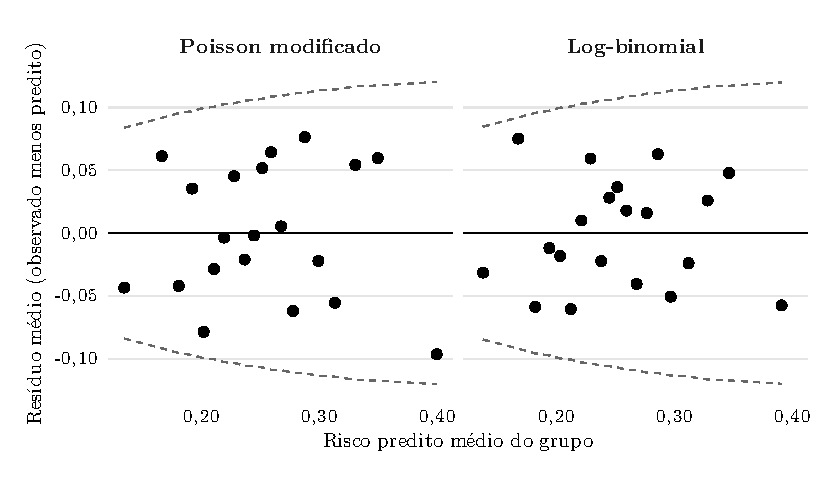
\includegraphics[width=0.85\textwidth]{fig_tcc_residuos_binados.eps}
  \caption{Resíduos binados, isto é, resíduo médio (evasão observada menos risco predito) em 20 grupos de mesmo tamanho formados pelo risco predito. As linhas tracejadas marcam $\pm$2 erros-padrão.}
  \label{fig:binados}
\end{figure}

\begin{figure}[H]
  \centering
  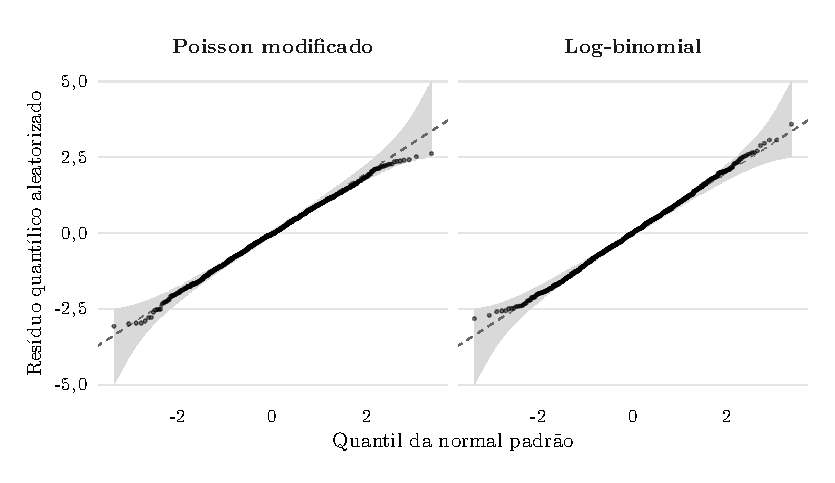
\includegraphics[width=0.85\textwidth]{fig_tcc_residuos_qq.eps}
  \caption{Gráfico quantil-quantil dos resíduos quantílicos aleatorizados em relação à normal padrão. A linha tracejada é a identidade e a faixa cinza, a banda simultânea de 95\%, sensível às caudas \citep{aldornoiman2013power}, dentro da qual uma amostra de valores independentes da normal padrão fica inteira em cerca de 95\% das vezes. Como os resíduos dependem dos coeficientes estimados, a banda serve de referência aproximada.}
  \label{fig:qq}
\end{figure}

\subsection*{Especificação do modelo principal}

A soma de quadrados não ponderada dos resíduos ficou próxima da esperada sob o modelo (p = 0,48). Nas simulações de \citet[p.~974]{hosmer1997comparison}, esse teste teve pouco poder contra ligação errada e interações omitidas, que o resultado não chega a afastar. O teste da ligação indicou desvio (p = 0,046). O coeficiente do quadrado do preditor linear foi negativo, sinal de que, nas matrículas de maior risco predito, o risco cresce menos do que a ligação logarítmica supõe. Nesse caso, os RR das categorias de maior risco, como a renda mais baixa, ficariam um pouco acima dos verdadeiros, direção em que vai também o log-binomial (Tabela~\ref{tab:logbin}). A troca da ligação, porém, não removeu o sinal, visto que, na regressão logística, o teste da ligação deu p = 0,079 e a log-verossimilhança diferiu da do Poisson modificado em 0,6, com o mesmo número de parâmetros. O quadrado do preditor linear costuma ser o termo mais sensível a desvios do modelo, sem indicar qual correção fazer \citep[p.~23]{pregibon1980goodness}. Em 1 SM em relação à mediana, o RR por padronização marginal foi o mesmo do modelo principal (1,27; 1,05--1,57). Em zero, ficou pouco abaixo (1,69, contra 1,73).

Nos resíduos parciais (Figura~\ref{fig:parciais}), as médias por faixa de renda acompanharam a curva do \textit{spline}, que cai até cerca de 3 SM e fica quase plana depois. Nas faixas acima de 10 SM, com poucas matrículas, as médias oscilaram em torno da curva com intervalos largos. Na nota, as médias dos 20 grupos se espalharam em torno da reta, sem curvatura. Só uma ficou a mais de dois erros-padrão dela, o esperado por acaso nesse número de grupos.

\begin{figure}[H]
  \centering
  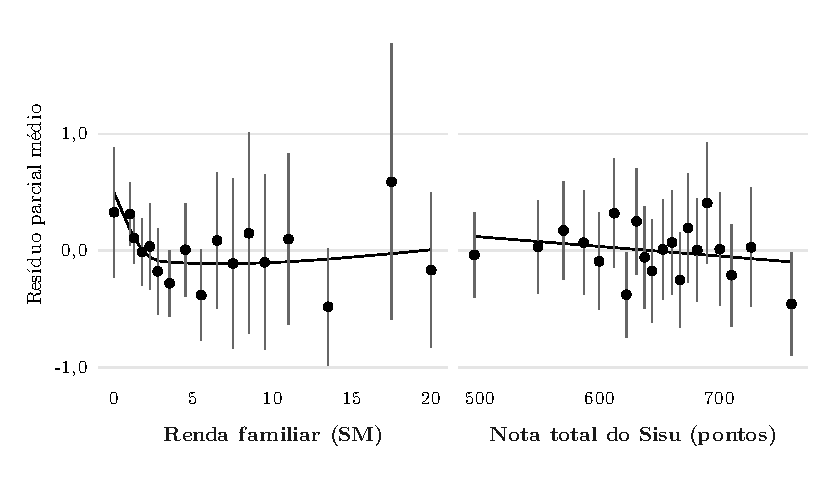
\includegraphics[width=0.85\textwidth]{fig_tcc_residuos_parciais.eps}
  \caption{Resíduos parciais da renda e da nota total do Sisu no Poisson modificado, na escala do log do risco. Os pontos são a média, em cada grupo, do resíduo de trabalho, $(y_i - \hat\pi_i)/\hat\pi_i$, somado à contribuição estimada da variável, com $\pm$2 erros-padrão. Os grupos são um por faixa de renda do questionário e 20 de mesmo tamanho na nota. A linha é a contribuição estimada pelo modelo. As médias por grupo substituem os pontos por matrícula porque, com desfecho binário, os resíduos individuais formam duas faixas sem leitura.}
  \label{fig:parciais}
\end{figure}


\begin{table}[H]
  \centering
  \caption{Fator generalizado de inflação da variância (GVIF) de cada termo do modelo principal, com a variância do modelo e com a HC3. $\text{GVIF}^{1/(2\,\text{gl})}$ se lê como o aumento médio do erro-padrão \citep{fox1992generalized}.}
  \label{tab:gvif}
  \tabela{tab_tcc_gvif.tex}
\end{table}

\subsection*{Formas da renda}

Com o mesmo modelo, mudou-se só o termo da renda (Tabela~\ref{tab:renda-formas}). O valor atribuído à faixa aberta não alterou o teste. O \textit{spline} teve AIC pouco acima do das três faixas da análise complementar. Com o ponto médio, 0,5 SM, na faixa de até 1 SM, a associação ficou mais forte e o teste caiu para p = 0,051, de modo que o valor de 1 SM do modelo principal é a escolha conservadora. A forma linear em SM, que impõe a mesma variação relativa do risco em toda a escala de renda, teve teste distante do limiar (p = 0,41). Das duas formas que dispensam o valor em SM, as 17 faixas como categorias diluíram a associação em 16 parâmetros, com o maior AIC. O escore ordinal, com as faixas numeradas de 0 a 16, deu p = 0,12 na forma linear e p = 0,054 em \textit{spline}. Os AIC das duas formas do escore ficaram praticamente iguais ao do \textit{spline} em SM, com diferença de até 1,2. Como os dados não preferem uma escala à outra, prevaleceu a do modelo principal, o \textit{spline} sobre o valor em SM, que usa a ordem e a distância entre as faixas.

\begin{table}[H]
  \centering
  \caption{Teste global da renda e AIC (verossimilhança de Bernoulli) segundo a forma da renda no modelo principal.}
  \label{tab:renda-formas}
  \tabela{tab_tcc_renda_formas.tex}
\end{table}

\subsection*{Renda por curso}

Os RR da faixa de até 1 SM em cada curso, mostrados na Figura~\ref{fig:renda-curso}, estão na Tabela~\ref{tab:renda-curso} com os números de matrículas e de evasões nessa faixa e nas rendas acima.

\begin{table}[H]
  \centering
  \caption{RR de evasão no primeiro ano da renda familiar de até 1 SM em relação às rendas acima, em cada curso, no modelo principal com a renda trocada pela faixa de até 1 SM e a interação dessa faixa com o curso (exploratório; $n = 1{.}312$).}
  \label{tab:renda-curso}
  \tabela{tab_tcc_renda_curso.tex}
\end{table}

\subsection*{Matrículas sem renda}

A imputação múltipla, que inclui as 8 matrículas sem renda, deu um teste da renda próximo ao dos casos completos (Tabela~\ref{tab:faltantes}). Atribuir a todas elas um mesmo valor extremo mostra até onde poderiam mover o teste, que iria de p = 0,068, se todas tivessem 20 SM, a p = 0,18, se todas tivessem renda zero. Em nenhum dos extremos o teste ficou abaixo de 0,05.

\begin{table}[H]
  \centering
  \caption{Teste global da renda segundo o tratamento das matrículas sem renda. A imputação usou 20 conjuntos e equações encadeadas, com teste combinado pela estatística $D_1$ \citep{li1991large}.}
  \label{tab:faltantes}
  \tabela{tab_tcc_faltantes.tex}
\end{table}


\subsection*{Discriminação}

A AUC corrigida de cada modelo resulta da aparente menos o otimismo estimado pelo \textit{bootstrap} (Tabela~\ref{tab:auc}). O ganho do modelo completo sobre a linha de base foi pequeno, com intervalo que incluiu zero.

\begin{table}[H]
  \centering
  \caption{Área sob a curva ROC (AUC) aparente e corrigida por otimismo, com o ganho
  em relação à linha de base ($\Delta$AUC), com IC 95\% por \textit{bootstrap}
  (5.000 reamostras, as mesmas para todos os modelos). Cada linha intermediária é
  a linha de base acrescida de um único bloco. Em uma simulação, os intervalos da AUC corrigida e do $\Delta$AUC cobriram o valor-alvo em 85\% e 91\% das amostras. O da AUC corrigida, quando errou, quase sempre ficou acima dele (Apêndice~\ref{apendice:comparacao}). O acréscimo do modelo
  completo foi testado pelo Wald conjunto (p = 0,12).}
  \label{tab:auc}
  \tabela{tab_art_auc.tex}
\end{table}

\subsection*{Cobertura dos intervalos da AUC}

Na simulação, que tomou as 1.312 matrículas como população e o risco do modelo completo como verdade, o intervalo do $\Delta$AUC cobriu o valor-alvo em 91\% das 200 amostras, com os erros divididos entre os dois lados (Tabela~\ref{tab:cobertura-auc}). O da AUC corrigida cobriu em 85\% e, quando errou, ficou quase sempre acima do alvo, porque a correção por \textit{bootstrap} deixou parte do otimismo (estimativa média de 0,584, contra alvo médio de 0,572). O limite superior desse intervalo tende, assim, a superestimar a discriminação. Essa verdade tem as associações estimadas, provavelmente mais fortes do que as reais. Os resultados descrevem o comportamento do método em um cenário parecido com estes dados, sem garantir a cobertura real. As 200 reamostras por amostra, contra 5.000 na análise principal, tornam os limites de cada intervalo simulado mais ruidosos.

\begin{table}[H]
  \centering
  \caption{Cobertura dos intervalos de 95\% da AUC corrigida e do $\Delta$AUC em uma simulação com 200 amostras e 200 reamostras cada. EP é o erro-padrão de Monte Carlo da cobertura e o alvo, a AUC do modelo ajustado na amostra avaliada na população.}
  \label{tab:cobertura-auc}
  \tabela{tab_tcc_cobertura_auc.tex}
\end{table}

\section{Escolaridade da mãe e faixa etária}
\label{apendice:mae-idade}

Nas 1.282 matrículas com as duas informações, acrescentar a escolaridade da mãe e a faixa etária ao modelo principal aproximou da referência as duas categorias de origem sem informação de escola, onde estão todos os ingressantes de 21 anos ou mais (Tabela~\ref{tab:mae-idade}). As demais estimativas variaram no máximo 0,07. Na coluna do modelo principal, a única diferença em relação à Tabela~\ref{tab:modelo} são as 30 matrículas sem escolaridade da mãe ou idade. A discriminação quase não mudou. Nessas matrículas, a AUC corrigida passou de 0,542 no modelo principal para 0,547 com as duas covariáveis.

\begin{table}[H]
  \centering
  \caption{RR do modelo principal e do modelo com escolaridade da mãe e faixa etária, nas mesmas 1.282 matrículas (324 evasões), pela regressão de Poisson modificada com variância HC3. Os dois modelos incluem também sexo, cor/raça, curso e coorte. Nas linhas da renda, da origem, da escolaridade da mãe e da faixa etária, o $p$ é o do teste global de Wald.}
  \label{tab:mae-idade}
  \tabela{tab_tcc_mae_idade.tex}
\end{table}

\clearpage
\section{Dicionário de variáveis}
\label{apendice:variaveis}

\begin{small}
\begin{longtable}{@{}>{\raggedright\arraybackslash}p{3.2cm}>{\raggedright\arraybackslash}p{8.0cm}>{\raggedright\arraybackslash}p{3.4cm}@{}}
  \caption{Variáveis utilizadas no estudo.}
  \label{tab:variaveis}\\
  \toprule
  Variável & Definição & Fonte \\
  \midrule
  \endfirsthead
  \toprule
  Variável & Definição & Fonte \\
  \midrule
  \endhead
  \bottomrule
  \endlastfoot
  Evasão no 1º ano & 1 se há desligamento (exceto conclusão e ajuste de currículo) com ano de evasão igual ao de ingresso; 0 caso contrário & Registro de desligamentos \\
  Evasão em 2 anos & como a anterior, com ano de evasão até o ano seguinte ao ingresso (sensibilidade) & Registro de desligamentos \\
  Trancamento no 1º ano & trancamento de curso registrado no ano de ingresso (sensibilidade) & Histórico acadêmico \\
  Sem registro no 1º semestre & nenhum lançamento no histórico do 1º semestre do ano de ingresso; saídas do 1º semestre nessa situação retiradas da base, exceto em 2020 (sensibilidade) & Histórico acadêmico \\
  Renda familiar & Q006 (17 faixas em SM); ponto médio da faixa (0 em nenhuma renda, 1 SM na faixa de até 1 SM e 20 SM na aberta); \textit{spline} natural com 3 gl; em faixas (até 1, 1 a 2, acima de 2 SM; a de até 1 SM inclui nenhuma renda) na análise complementar & Questionário do Enem \\
  Renda per capita & ponto médio da faixa dividido pelo número de moradores (Q005); em \textit{spline} e até 1,5 SM (sensibilidade) & Questionário do Enem \\
  Nota total Sisu & média ponderada das cinco provas pelos pesos do curso, por 100 pontos & Cadastro Sisu \\
  Notas MT e CN & Matemática e Ciências da Natureza, por 100 pontos (análise complementar) & Microdados do Enem \\
  Origem & modalidade de ingresso combinada à dependência administrativa da escola (6 categorias) & Cadastro Sisu; microdados do Enem \\
  Vaga reservada com critério de renda & ingresso por vaga reservada com critério de renda, pelo código da modalidade no cadastro, separado da reserva sem esse critério; descritivo (Tabela~\ref{tab:renda-origem}) e sensibilidade & Cadastro Sisu \\
  Sexo; cor/raça & conforme declarado na inscrição do Enem & Microdados do Enem \\
  Escolaridade da mãe & até médio incompleto, médio completo, superior (sensibilidade) & Questionário do Enem \\
  Faixa etária & até 18, 19--20, 21 anos ou mais (sensibilidade) & Microdados do Enem \\
  Curso & Estatística; Física, Matemática e Química, bacharelado e licenciatura & Cadastro Sisu \\
  Coorte & ano de ingresso (2019--2024) & Cadastro Sisu \\
  Reprovação por frequência e por nota & ao menos uma disciplina no 1º semestre (descritivo, Tabelas~\ref{tab:coorte} e~\ref{tab:reprovacao}) & Histórico acadêmico \\
\end{longtable}
\end{small}


\section{Fluxo de análise}
\label{apendice:pipeline}

Os \textit{scripts} abaixo geram todos os números, tabelas e figuras deste trabalho a partir das bases cedidas pela Prograd, dos microdados do Enem e dos indicadores de trajetória do Inep. As bases da Ufes, que contêm identificadores pessoais, não são divulgadas. O código está no repositório \url{https://github.com/cheriroga/tcc-evasao-cce}, de acesso restrito, liberado mediante solicitação à autora.

\begin{table}[H]
  \centering
  \caption{Fluxo de análise.}
  \label{tab:scripts}
  \begin{tabular}{>{\raggedright\arraybackslash}p{5.0cm} >{\raggedright\arraybackslash}p{9.5cm}}
    \toprule
    Script & Função \\
    \midrule
    \texttt{00\_util.R} & caminhos, funções comuns e definição das variáveis \\
    \texttt{01\_filtra\_enem.py}, \texttt{02\_liga\_enem.R} & ligação do cadastro Sisu aos microdados do Enem pela coincidência das cinco notas \\
    \texttt{03\_base\_analitica.R} & ligação das bases da Ufes, construção do desfecho e das variáveis do histórico \\
    \texttt{04\_descritiva.R} & descrição, composição do corpo discente, comparação com a Ufes e fluxo de seleção \\
    \texttt{05\_modelo.R} & modelo principal, discriminação, sensibilidades, análises complementares e comparação de modelos (Apêndice~\ref{apendice:comparacao}) \\
    \texttt{06\_inep\_trajetoria.R} & indicadores de trajetória do Inep para os cursos do CCE e para as federais (Desfecho e Conclusão) \\
    \texttt{07\_q006\_nacional.sh} & distribuição da renda familiar (Q006) entre os inscritos do Enem, por edição \\
    \texttt{08\_tabelas\_figuras.R} & tabelas e figuras \\
    \texttt{09\_erro\_monte\_carlo.R} & variação dos limites dos intervalos da AUC entre sementes do \textit{bootstrap} \\
    \texttt{10\_cobertura\_auc.R} & cobertura dos intervalos da AUC corrigida e do $\Delta$AUC, por simulação (Apêndice~\ref{apendice:comparacao}) \\
    \texttt{11\_formas\_hc.R} & erros-padrão e testes globais do modelo principal com as formas HC0 a HC3 \\
    \bottomrule
  \end{tabular}
\end{table}


\section{Lista de verificação STROBE}
\label{apendice:strobe}

Os 22 itens da lista de verificação STROBE para estudos de coorte são tratados no texto, salvo dois que não se aplicam a este desenho (Tabela~\ref{tab:strobe}), uma vez que o estudo não usa pareamento e o seguimento pelo registro de desligamentos não tem perdas. As recomendações estão resumidas da tradução de \citet{malta2010strobe}. Como a lista registra só onde cada item é relatado, ela não avalia a qualidade do estudo, uso que os próprios autores da declaração descartam \citep{vonelm2007strobe}.

{\small
\begin{longtable}{>{\raggedright\arraybackslash}p{0.8cm} >{\raggedright\arraybackslash}p{7.0cm} >{\raggedright\arraybackslash}p{6.5cm}}
  \caption{Lista de verificação STROBE para estudos de coorte e lugar do texto em que cada item é tratado. Recomendações resumidas de \citet{malta2010strobe}. Nos itens 8, 13, 14 e 15, a lista pede a informação separada por grupo de exposição; as taxas por categoria de cada covariável estão na Tabela~\ref{tab:descritiva}.}
  \label{tab:strobe} \\
    \toprule
    Item & Recomendação & Onde no texto \\
    \midrule
  \endfirsthead
    \toprule
    Item & Recomendação & Onde no texto \\
    \midrule
  \endhead
    \bottomrule
  \endlastfoot
    \multicolumn{3}{l}{\textit{Título e resumo}} \\
    1a & Indicar o desenho do estudo no título ou no resumo, com termo de uso comum & Resumo \\
    1b & Resumo informativo e equilibrado do que foi feito e do que foi encontrado & Resumo \\
    \multicolumn{3}{l}{\textit{Introdução}} \\
    2 & Referencial teórico e razões para a pesquisa & Seções~\ref{sec:introducao} e~\ref{sec:fundamentacao} \\
    3 & Objetivos específicos, incluindo hipóteses prévias & Seção~\ref{sec:introducao}; sem hipótese direcional \\
    \multicolumn{3}{l}{\textit{Métodos}} \\
    4 & Elementos-chave do desenho no início do texto & Seção~\ref{sec:delineamento} \\
    5 & Contexto, locais e datas de recrutamento, exposição, acompanhamento e coleta & Seções~\ref{sec:delineamento}, \ref{sec:fontes} e~\ref{sec:desfecho} \\
    6a & Critérios de elegibilidade, fontes e métodos de seleção; métodos de acompanhamento & Seções~\ref{sec:elegibilidade} e~\ref{sec:desfecho}; Figura~\ref{fig:fluxograma} \\
    6b & Em estudos pareados, critérios de pareamento e número de expostos e não expostos & Não se aplica: sem pareamento \\
    7 & Definição de desfechos, exposições, preditores, confundidores e modificadores de efeito & Seções~\ref{sec:desfecho} e~\ref{sec:covariaveis}; Apêndice~\ref{apendice:variaveis} \\
    8 & Fonte dos dados e método de mensuração de cada variável & Seção~\ref{sec:fontes}; Apêndice~\ref{apendice:variaveis}; Anexo~A \\
    9 & Medidas adotadas diante de potenciais fontes de viés & Seções~\ref{sec:verificacoes} e~\ref{sec:sensibilidade} \\
    10 & Como se chegou ao tamanho do estudo & Seção~\ref{sec:modelo}, Equação~\eqref{eq:poder} \\
    11 & Tratamento das variáveis quantitativas; categorizações adotadas e por quê & Seções~\ref{sec:covariaveis} e~\ref{sec:modelo}; Apêndice~\ref{apendice:comparacao} \\
    12a & Métodos estatísticos, incluindo os de controle de confundimento & Seção~\ref{sec:fund-estatistica} e Seções~\ref{sec:modelo} a~\ref{sec:verificacoes} \\
    12b & Métodos para examinar subgrupos e interações & Seção~\ref{sec:modelo} (nota $\times$ curso) e~\ref{sec:sensibilidade} (renda $\times$ tipo de coorte) \\
    12c & Tratamento dos dados ausentes & Seções~\ref{sec:fund-ausentes} e~\ref{sec:ausentes} \\
    12d & Tratamento das perdas de acompanhamento & Não se aplica: o registro cobre o primeiro ano de todas as coortes (Seção~\ref{sec:desfecho}) \\
    12e & Análises de sensibilidade & Seção~\ref{sec:sensibilidade} \\
    \multicolumn{3}{l}{\textit{Resultados}} \\
    13a & Número de participantes em cada etapa & Seção~\ref{sec:elegibilidade}; Figura~\ref{fig:fluxograma} \\
    13b & Razões das exclusões em cada etapa & Seção~\ref{sec:elegibilidade}; Figura~\ref{fig:fluxograma} \\
    13c & Diagrama de fluxo & Figura~\ref{fig:fluxograma} \\
    14a & Características dos participantes e informação sobre exposições e confundidores & Tabelas~\ref{tab:descritiva}, \ref{tab:coorte}, \ref{tab:renda-origem} e~\ref{tab:composicao} \\
    14b & Número de participantes com dados ausentes em cada variável & Seção~\ref{sec:elegibilidade} (renda) e~\ref{sec:sensibilidade} (escolaridade da mãe e faixa etária) \\
    14c & Período de acompanhamento & Seção~\ref{sec:desfecho}: um ano acadêmico em todas as coortes \\
    15 & Número de eventos ao longo do tempo & Tabelas~\ref{tab:descritiva} e~\ref{tab:coorte} \\
    16a & Estimativas não ajustadas e ajustadas, com precisão; confundidores do ajuste e por quê & Tabelas~\ref{tab:descritiva} (taxas brutas) e~\ref{tab:modelo}; Seção~\ref{sec:modelo} \\
    16b & Pontos de corte das variáveis contínuas categorizadas & Seções~\ref{sec:covariaveis} e~\ref{sec:sensibilidade}; Tabela~\ref{tab:descritiva} \\
    16c & Se pertinente, risco absoluto em um período relevante & Tabela~\ref{tab:descritiva} (taxa de evasão no primeiro ano por categoria) \\
    17 & Outras análises: subgrupos, interações, sensibilidade & Tabelas~\ref{tab:sensibilidade}, \ref{tab:renda-coortes} e~\ref{tab:complementar}; Apêndices~\ref{apendice:comparacao} e~\ref{apendice:mae-idade} \\
    \multicolumn{3}{l}{\textit{Discussão}} \\
    18 & Principais achados em relação aos objetivos & Seções~\ref{sec:discussao} e~\ref{sec:conclusao} \\
    19 & Limitações, com a direção e a magnitude dos vieses & Seção~\ref{sec:disc-limitacoes} \\
    20 & Interpretação cautelosa, considerando limitações, multiplicidade e outros estudos & Seção~\ref{sec:discussao}; multiplicidade nas Seções~\ref{sec:fund-testes} e~\ref{sec:modelo} \\
    21 & Generalização (validade externa) & Seção~\ref{sec:disc-limitacoes} \\
    \multicolumn{3}{l}{\textit{Outras informações}} \\
    22 & Fonte de financiamento e papel dos financiadores & Seção~\ref{sec:software} \\
\end{longtable}
}

% ==============================================================================
% X. ANEXOS
% ==============================================================================
\clearpage
\section*{Anexos}
\addcontentsline{toc}{section}{Anexos}

\section*{Anexo A -- Questão Q006 do questionário socioeconômico do Enem}
\addcontentsline{toc}{section}{Anexo A -- Questão Q006 do questionário socioeconômico do Enem}

Enunciado e alternativas conforme o Dicionário de Microdados do ENEM 2023
(Inep). Nas edições de 2017 a 2022, também usadas neste trabalho, as faixas são as
mesmas, expressas em múltiplos do salário mínimo informado no questionário de
cada edição.

\begin{quote}
\textit{Q006. Qual é a renda mensal de sua família? (Some a sua renda com a dos
seus familiares.)}
\end{quote}

\begin{small}
\begin{longtable}{@{}l l l@{}}
  \caption{Alternativas da questão Q006 (Enem 2023) e equivalência em salários mínimos.}
  \label{tab:q006}\\
  \toprule
  Alternativa & Texto (Enem 2023) & Faixa em salários mínimos \\
  \midrule
  \endfirsthead
  \toprule
  Alternativa & Texto (Enem 2023) & Faixa em salários mínimos \\
  \midrule
  \endhead
  \bottomrule
  \endlastfoot
  A & Nenhuma Renda & 0 \\
  B & Até R\$ 1.320,00 & até 1 \\
  C & De R\$ 1.320,01 até R\$ 1.980,00 & 1 a 1,5 \\
  D & De R\$ 1.980,01 até R\$ 2.640,00 & 1,5 a 2 \\
  E & De R\$ 2.640,01 até R\$ 3.300,00 & 2 a 2,5 \\
  F & De R\$ 3.300,01 até R\$ 3.960,00 & 2,5 a 3 \\
  G & De R\$ 3.960,01 até R\$ 5.280,00 & 3 a 4 \\
  H & De R\$ 5.280,01 até R\$ 6.600,00 & 4 a 5 \\
  I & De R\$ 6.600,01 até R\$ 7.920,00 & 5 a 6 \\
  J & De R\$ 7.920,01 até R\$ 9.240,00 & 6 a 7 \\
  K & De R\$ 9.240,01 até R\$ 10.560,00 & 7 a 8 \\
  L & De R\$ 10.560,01 até R\$ 11.880,00 & 8 a 9 \\
  M & De R\$ 11.880,01 até R\$ 13.200,00 & 9 a 10 \\
  N & De R\$ 13.200,01 até R\$ 15.840,00 & 10 a 12 \\
  O & De R\$ 15.840,01 até R\$ 19.800,00 & 12 a 15 \\
  P & De R\$ 19.800,01 até R\$ 26.400,00 & 15 a 20 \\
  Q & Acima de R\$ 26.400,00 & mais de 20 \\
\end{longtable}
\end{small}

\section*{Anexo B -- Registro acadêmico do primeiro semestre de 2020}
\addcontentsline{toc}{section}{Anexo B -- Registro acadêmico do primeiro semestre de 2020}

Trecho do Ofício Circular nº 16/2020/Gabinete/Prograd/UFES, de 21 de agosto de
2020, que detalha procedimentos da Resolução nº 30/2020 do Conselho de Ensino,
Pesquisa e Extensão \citep{ufes2020oficio16}:

\begin{quote}
\textbf{Registro de notas e cancelamento de disciplinas do primeiro semestre
letivo regular}

-- Os(as) estudantes matriculados em disciplinas do primeiro semestre letivo
regular de 2020, que não as tenham concluído, não deverão ter registro de nota
efetuado.

-- Os(as) estudantes sem registro de nota terão sua matrícula na disciplina
cancelada pela Prograd assim que encerrado o período para digitação das pautas
finais.

-- Serão canceladas pela Prograd, na oferta do semestre 2020/1, todas as
disciplinas cujas realizações foram vedadas pela Resolução n.º 07/2020 do
Conselho Universitário.

[\ldots]

\textbf{Ofertas de disciplinas no primeiro semestre letivo especial}

-- Para fins de registro nos sistemas acadêmicos, as disciplinas ofertadas no
primeiro semestre letivo especial de 2020 utilizarão como parâmetro o semestre
2020/1, cujas datas de início e término de período encontram-se devidamente
atualizadas.
\end{quote}

\end{document}
